\documentclass[twoside]{book}

% Packages required by doxygen
\usepackage{fixltx2e}
\usepackage{calc}
\usepackage{doxygen}
\usepackage[export]{adjustbox} % also loads graphicx
\usepackage{graphicx}
\usepackage[utf8]{inputenc}
\usepackage{makeidx}
\usepackage{multicol}
\usepackage{multirow}
\PassOptionsToPackage{warn}{textcomp}
\usepackage{textcomp}
\usepackage[nointegrals]{wasysym}
\usepackage[table]{xcolor}

% Font selection
\usepackage[T1]{fontenc}
\usepackage[scaled=.90]{helvet}
\usepackage{courier}
\usepackage{amssymb}
\usepackage{sectsty}
\renewcommand{\familydefault}{\sfdefault}
\allsectionsfont{%
  \fontseries{bc}\selectfont%
  \color{darkgray}%
}
\renewcommand{\DoxyLabelFont}{%
  \fontseries{bc}\selectfont%
  \color{darkgray}%
}
\newcommand{\+}{\discretionary{\mbox{\scriptsize$\hookleftarrow$}}{}{}}

% Page & text layout
\usepackage{geometry}
\geometry{%
  a4paper,%
  top=2.5cm,%
  bottom=2.5cm,%
  left=2.5cm,%
  right=2.5cm%
}
\tolerance=750
\hfuzz=15pt
\hbadness=750
\setlength{\emergencystretch}{15pt}
\setlength{\parindent}{0cm}
\setlength{\parskip}{3ex plus 2ex minus 2ex}
\makeatletter
\renewcommand{\paragraph}{%
  \@startsection{paragraph}{4}{0ex}{-1.0ex}{1.0ex}{%
    \normalfont\normalsize\bfseries\SS@parafont%
  }%
}
\renewcommand{\subparagraph}{%
  \@startsection{subparagraph}{5}{0ex}{-1.0ex}{1.0ex}{%
    \normalfont\normalsize\bfseries\SS@subparafont%
  }%
}
\makeatother

% Headers & footers
\usepackage{fancyhdr}
\pagestyle{fancyplain}
\fancyhead[LE]{\fancyplain{}{\bfseries\thepage}}
\fancyhead[CE]{\fancyplain{}{}}
\fancyhead[RE]{\fancyplain{}{\bfseries\leftmark}}
\fancyhead[LO]{\fancyplain{}{\bfseries\rightmark}}
\fancyhead[CO]{\fancyplain{}{}}
\fancyhead[RO]{\fancyplain{}{\bfseries\thepage}}
\fancyfoot[LE]{\fancyplain{}{}}
\fancyfoot[CE]{\fancyplain{}{}}
\fancyfoot[RE]{\fancyplain{}{\bfseries\scriptsize Generated by Doxygen }}
\fancyfoot[LO]{\fancyplain{}{\bfseries\scriptsize Generated by Doxygen }}
\fancyfoot[CO]{\fancyplain{}{}}
\fancyfoot[RO]{\fancyplain{}{}}
\renewcommand{\footrulewidth}{0.4pt}
\renewcommand{\chaptermark}[1]{%
  \markboth{#1}{}%
}
\renewcommand{\sectionmark}[1]{%
  \markright{\thesection\ #1}%
}

% Indices & bibliography
\usepackage{natbib}
\usepackage[titles]{tocloft}
\setcounter{tocdepth}{3}
\setcounter{secnumdepth}{5}
\makeindex

% Hyperlinks (required, but should be loaded last)
\usepackage{ifpdf}
\ifpdf
  \usepackage[pdftex,pagebackref=true]{hyperref}
\else
  \usepackage[ps2pdf,pagebackref=true]{hyperref}
\fi
\hypersetup{%
  colorlinks=true,%
  linkcolor=blue,%
  citecolor=blue,%
  unicode%
}

% Custom commands
\newcommand{\clearemptydoublepage}{%
  \newpage{\pagestyle{empty}\cleardoublepage}%
}

\usepackage{caption}
\captionsetup{labelsep=space,justification=centering,font={bf},singlelinecheck=off,skip=4pt,position=top}

%===== C O N T E N T S =====

\begin{document}

% Titlepage & ToC
\hypersetup{pageanchor=false,
             bookmarksnumbered=true,
             pdfencoding=unicode
            }
\pagenumbering{alph}
\begin{titlepage}
\vspace*{7cm}
\begin{center}%
{\Large Atila\+Calculator\+Software \\[1ex]\large 2.\+0.\+0 }\\
\vspace*{1cm}
{\large Generated by Doxygen 1.8.13}\\
\end{center}
\end{titlepage}
\clearemptydoublepage
\pagenumbering{roman}
\tableofcontents
\clearemptydoublepage
\pagenumbering{arabic}
\hypersetup{pageanchor=true}

%--- Begin generated contents ---
\chapter{Atila\+Calculator\+Software}
\label{index}\hypertarget{index}{}
\begin{DoxyItemize}
\item \href{https://www.boost.org/}{\tt Boost} 1.\+72
\item \href{https://www.gidhome.com/gid-plus/tools/476/gidpost/}{\tt Gi\+D\+Post} 2.\+7
\item \href{https://zlib.net/}{\tt zlib}
\item \href{https://portal.hdfgroup.org/pages/viewpage.action?pageId=50073884}{\tt H\+D\+F5 Library}
\item \href{https://vtk.org/}{\tt V\+TK}, tested with versions\+:
\begin{DoxyItemize}
\item 9.\+0.\+1
\item 9.\+0.\+0
\item 8.\+2.\+0
\item 8.\+1.\+2
\item 8.\+1.\+1
\item 8.\+0.\+1
\item 8.\+0.\+0
\item 7.\+1.\+0
\end{DoxyItemize}
\end{DoxyItemize}


\begin{DoxyCode}
mkdir build && cd build
cmake ../ # or cmake -DVTK\_DIR:PATH=/path/to/vtk ../ -Wno-dev
make
./AtilaCalculatorSoftware # or ./AtilaCalculatorSoftware /path/to/data/directory
\end{DoxyCode}


or using make


\begin{DoxyCode}
make run
\end{DoxyCode}


See the \href{https://github.com/Xisabla/AtilaCalculatorSoftware/projects}{\tt project management} tab

To apply an enhancement idea, open \href{https://github.com/Xisabla/AtilaCalculatorSoftware/issues}{\tt an issue}. Describe the wanted feature as much as possible.

To add a new feature/enhancement\+:
\begin{DoxyItemize}
\item \href{https://github.com/Xisabla/AtilaCalculatorSoftware/issues}{\tt Open an issue} as described above
\item Add to your issue a detailed description (needed methods, objects, behavior, ...) (a marked list is always a good idea)
\item Add your enhancement issue to the \href{https://github.com/Xisabla/AtilaCalculatorSoftware/projects/2}{\tt {\ttfamily Features} project} as a \char`\"{}\+To Do\char`\"{} item
\item Open a new branch {\ttfamily feature/$<$feature-\/name$>$}
\item Once the development part is over, perform a \href{https://github.com/Xisabla/AtilaCalculatorSoftware/pulls}{\tt pull request} from your feature developing branch and do not forget to update the project \href{https://github.com/Xisabla/AtilaCalculatorSoftware/blob/master/include/version.h}{\tt version}
\end{DoxyItemize}

Project under ./\+L\+I\+C\+E\+N\+SE.md \char`\"{}\+M\+I\+T License\char`\"{} 
\chapter{Hierarchical Index}
\section{Class Hierarchy}
This inheritance list is sorted roughly, but not completely, alphabetically\+:\begin{DoxyCompactList}
\item \contentsline{section}{Binary\+Data}{\pageref{classBinaryData}}{}
\begin{DoxyCompactList}
\item \contentsline{section}{Binary\+Data\+Wrapper}{\pageref{classBinaryDataWrapper}}{}
\end{DoxyCompactList}
\item Main\+Window\begin{DoxyCompactList}
\item \contentsline{section}{Main\+Window}{\pageref{classMainWindow}}{}
\end{DoxyCompactList}
\item \contentsline{section}{Mesh}{\pageref{classMesh}}{}
\item \contentsline{section}{Node}{\pageref{classNode}}{}
\item Q\+Main\+Window\begin{DoxyCompactList}
\item \contentsline{section}{Main\+Window}{\pageref{classMainWindow}}{}
\end{DoxyCompactList}
\item \contentsline{section}{Result}{\pageref{classResult}}{}
\end{DoxyCompactList}

\chapter{Class Index}
\section{Class List}
Here are the classes, structs, unions and interfaces with brief descriptions\+:\begin{DoxyCompactList}
\item\contentsline{section}{\hyperlink{classBinaryData}{Binary\+Data} \\*Load the resources file and allow to read meshes and results from it }{\pageref{classBinaryData}}{}
\item\contentsline{section}{\hyperlink{classBinaryDataWrapper}{Binary\+Data\+Wrapper} \\*Wrapper around the \hyperlink{classBinaryData}{Binary\+Data} class that allows to interact with V\+TK }{\pageref{classBinaryDataWrapper}}{}
\item\contentsline{section}{\hyperlink{classMainWindow}{Main\+Window} \\*Qt main window }{\pageref{classMainWindow}}{}
\item\contentsline{section}{\hyperlink{classMesh}{Mesh} \\*Representation of a mesh, all of its nodes and elements }{\pageref{classMesh}}{}
\item\contentsline{section}{\hyperlink{classNode}{Node} \\*Point in 3D space representation, part of a \hyperlink{classMesh}{Mesh} }{\pageref{classNode}}{}
\item\contentsline{section}{\hyperlink{classResult}{Result} \\*Representation of all the results and their components read from a res file }{\pageref{classResult}}{}
\end{DoxyCompactList}

\chapter{File Index}
\section{File List}
Here is a list of all files with brief descriptions\+:\begin{DoxyCompactList}
\item\contentsline{section}{include/\hyperlink{binary__data_8h}{binary\+\_\+data.\+h} }{\pageref{binary__data_8h}}{}
\item\contentsline{section}{include/\hyperlink{binary__data__wrapper_8h}{binary\+\_\+data\+\_\+wrapper.\+h} }{\pageref{binary__data__wrapper_8h}}{}
\item\contentsline{section}{include/\hyperlink{main__window_8h}{main\+\_\+window.\+h} }{\pageref{main__window_8h}}{}
\item\contentsline{section}{include/\hyperlink{mesh_8h}{mesh.\+h} }{\pageref{mesh_8h}}{}
\item\contentsline{section}{include/\hyperlink{result_8h}{result.\+h} }{\pageref{result_8h}}{}
\item\contentsline{section}{include/\hyperlink{utilities_8h}{utilities.\+h} }{\pageref{utilities_8h}}{}
\item\contentsline{section}{include/\hyperlink{version_8h}{version.\+h} }{\pageref{version_8h}}{}
\item\contentsline{section}{src/\hyperlink{app_8cpp}{app.\+cpp} }{\pageref{app_8cpp}}{}
\item\contentsline{section}{src/\hyperlink{binary__data_8cpp}{binary\+\_\+data.\+cpp} }{\pageref{binary__data_8cpp}}{}
\item\contentsline{section}{src/\hyperlink{binary__data__wrapper_8cpp}{binary\+\_\+data\+\_\+wrapper.\+cpp} }{\pageref{binary__data__wrapper_8cpp}}{}
\item\contentsline{section}{src/\hyperlink{main__window_8cpp}{main\+\_\+window.\+cpp} }{\pageref{main__window_8cpp}}{}
\item\contentsline{section}{src/\hyperlink{mesh_8cpp}{mesh.\+cpp} }{\pageref{mesh_8cpp}}{}
\item\contentsline{section}{src/\hyperlink{result_8cpp}{result.\+cpp} }{\pageref{result_8cpp}}{}
\item\contentsline{section}{src/\hyperlink{utilities_8cpp}{utilities.\+cpp} }{\pageref{utilities_8cpp}}{}
\end{DoxyCompactList}

\chapter{Class Documentation}
\hypertarget{classBinaryData}{}\section{Binary\+Data Class Reference}
\label{classBinaryData}\index{Binary\+Data@{Binary\+Data}}


Load the resources file and allow to read meshes and results from it.  




{\ttfamily \#include $<$binary\+\_\+data.\+h$>$}

Inheritance diagram for Binary\+Data\+:\begin{figure}[H]
\begin{center}
\leavevmode
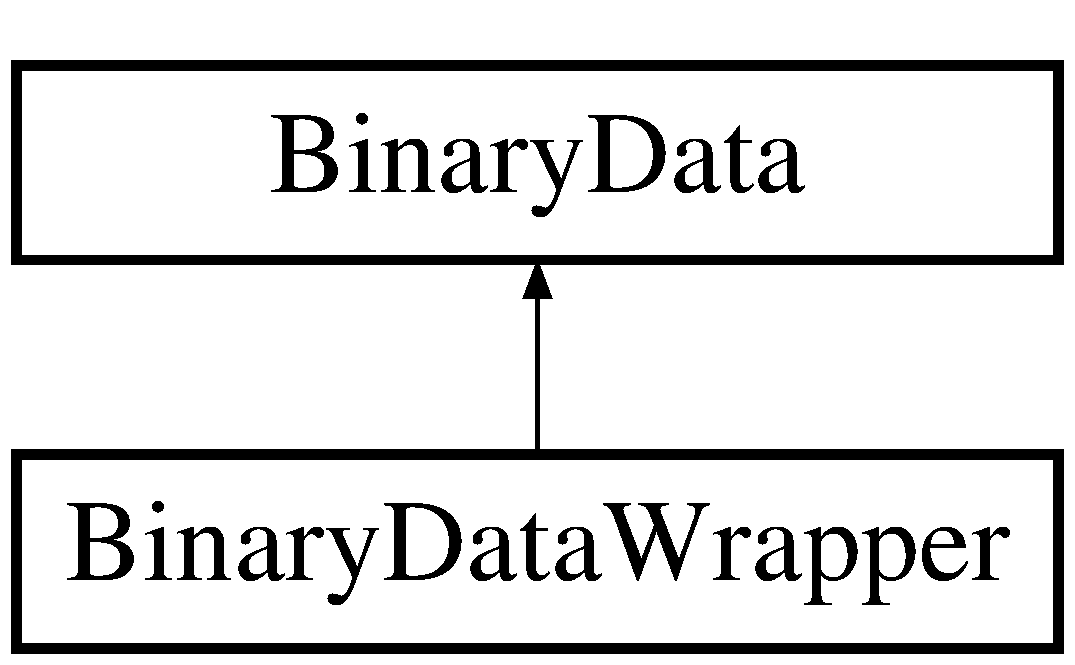
\includegraphics[height=2.000000cm]{dc/d47/classBinaryData}
\end{center}
\end{figure}
\subsection*{Public Member Functions}
\begin{DoxyCompactItemize}
\item 
\hyperlink{classBinaryData_a0bba582d92f95dc186e3c36ea9ddcd36}{Binary\+Data} (const std\+::string \&\hyperlink{classBinaryData_a9eae74bdf3b91a3e1461802d820591e3}{file})
\item 
gz\+File \hyperlink{classBinaryData_a20d3521069ee75c21b83de91ddf5c44b}{get\+File} ()
\item 
std\+::vector$<$ \hyperlink{classMesh}{Mesh} $>$ \& \hyperlink{classBinaryData_ac2baca71c75e2ea6d12ed89d265dfb6f}{get\+Meshes} ()
\item 
std\+::vector$<$ \hyperlink{classResult}{Result} $>$ \& \hyperlink{classBinaryData_a33f15e0f1b9c34d286e84bc615e7a83e}{get\+Results} ()
\item 
\hyperlink{classBinaryData_a31499383f285646922658e87866a73ea}{$\sim$\+Binary\+Data} ()
\begin{DoxyCompactList}\small\item\em Closes open files. \end{DoxyCompactList}\item 
void \hyperlink{classBinaryData_a11126f35f2b4f20edc1f3c36f549fb10}{read\+Meshes} ()
\item 
std\+::optional$<$ \hyperlink{classResult}{Result} $>$ \hyperlink{classBinaryData_aa2fad71246ba4648b6f9d2045fd4201e}{read\+Result} ()
\begin{DoxyCompactList}\small\item\em Read one result from the res gz\+File. \end{DoxyCompactList}\item 
std\+::vector$<$ \hyperlink{classResult}{Result} $>$ \hyperlink{classBinaryData_a0faec96c84437c29694d2e54689b7f07}{read\+Results} (unsigned int n=0)
\begin{DoxyCompactList}\small\item\em Read the n given results, stops if there is no more result. \end{DoxyCompactList}\end{DoxyCompactItemize}
\subsection*{Protected Attributes}
\begin{DoxyCompactItemize}
\item 
gz\+File \hyperlink{classBinaryData_a9eae74bdf3b91a3e1461802d820591e3}{file}
\begin{DoxyCompactList}\small\item\em Opened res gz\+File. \end{DoxyCompactList}\item 
std\+::vector$<$ \hyperlink{classMesh}{Mesh} $>$ \hyperlink{classBinaryData_af5e37d66b40c5cc7d835bac81a165b14}{meshes}
\begin{DoxyCompactList}\small\item\em Read meshes. \end{DoxyCompactList}\item 
std\+::vector$<$ \hyperlink{classResult}{Result} $>$ \hyperlink{classBinaryData_a81c3bb02cb37946f441ce336bdf43784}{results}
\begin{DoxyCompactList}\small\item\em Read meshes. \end{DoxyCompactList}\end{DoxyCompactItemize}
\subsection*{Static Protected Attributes}
\begin{DoxyCompactItemize}
\item 
static const int \hyperlink{classBinaryData_a4e95a7b65e2fa6374d92108bb90eaf5b}{byte\+Order\+Check} = 0x91d
\begin{DoxyCompactList}\small\item\em Constant value for reading check. \end{DoxyCompactList}\end{DoxyCompactItemize}


\subsection{Detailed Description}
Load the resources file and allow to read meshes and results from it. 

\subsection{Constructor \& Destructor Documentation}
\mbox{\Hypertarget{classBinaryData_a0bba582d92f95dc186e3c36ea9ddcd36}\label{classBinaryData_a0bba582d92f95dc186e3c36ea9ddcd36}} 
\index{Binary\+Data@{Binary\+Data}!Binary\+Data@{Binary\+Data}}
\index{Binary\+Data@{Binary\+Data}!Binary\+Data@{Binary\+Data}}
\subsubsection{\texorpdfstring{Binary\+Data()}{BinaryData()}}
{\footnotesize\ttfamily Binary\+Data\+::\+Binary\+Data (\begin{DoxyParamCaption}\item[{const std\+::string \&}]{file }\end{DoxyParamCaption})}


\begin{DoxyParams}{Parameters}
{\em file} & Path to the res gz\+File \\
\hline
\end{DoxyParams}
\mbox{\Hypertarget{classBinaryData_a31499383f285646922658e87866a73ea}\label{classBinaryData_a31499383f285646922658e87866a73ea}} 
\index{Binary\+Data@{Binary\+Data}!````~Binary\+Data@{$\sim$\+Binary\+Data}}
\index{````~Binary\+Data@{$\sim$\+Binary\+Data}!Binary\+Data@{Binary\+Data}}
\subsubsection{\texorpdfstring{$\sim$\+Binary\+Data()}{~BinaryData()}}
{\footnotesize\ttfamily Binary\+Data\+::$\sim$\+Binary\+Data (\begin{DoxyParamCaption}{ }\end{DoxyParamCaption})}



Closes open files. 



\subsection{Member Function Documentation}
\mbox{\Hypertarget{classBinaryData_a20d3521069ee75c21b83de91ddf5c44b}\label{classBinaryData_a20d3521069ee75c21b83de91ddf5c44b}} 
\index{Binary\+Data@{Binary\+Data}!get\+File@{get\+File}}
\index{get\+File@{get\+File}!Binary\+Data@{Binary\+Data}}
\subsubsection{\texorpdfstring{get\+File()}{getFile()}}
{\footnotesize\ttfamily gz\+File Binary\+Data\+::get\+File (\begin{DoxyParamCaption}{ }\end{DoxyParamCaption})}

\begin{DoxyReturn}{Returns}
The currently open res gz\+File 
\end{DoxyReturn}
\mbox{\Hypertarget{classBinaryData_ac2baca71c75e2ea6d12ed89d265dfb6f}\label{classBinaryData_ac2baca71c75e2ea6d12ed89d265dfb6f}} 
\index{Binary\+Data@{Binary\+Data}!get\+Meshes@{get\+Meshes}}
\index{get\+Meshes@{get\+Meshes}!Binary\+Data@{Binary\+Data}}
\subsubsection{\texorpdfstring{get\+Meshes()}{getMeshes()}}
{\footnotesize\ttfamily std\+::vector$<$ \hyperlink{classMesh}{Mesh} $>$ \& Binary\+Data\+::get\+Meshes (\begin{DoxyParamCaption}{ }\end{DoxyParamCaption})}

\begin{DoxyReturn}{Returns}
The loaded meshes 
\end{DoxyReturn}
\mbox{\Hypertarget{classBinaryData_a33f15e0f1b9c34d286e84bc615e7a83e}\label{classBinaryData_a33f15e0f1b9c34d286e84bc615e7a83e}} 
\index{Binary\+Data@{Binary\+Data}!get\+Results@{get\+Results}}
\index{get\+Results@{get\+Results}!Binary\+Data@{Binary\+Data}}
\subsubsection{\texorpdfstring{get\+Results()}{getResults()}}
{\footnotesize\ttfamily std\+::vector$<$ \hyperlink{classResult}{Result} $>$ \& Binary\+Data\+::get\+Results (\begin{DoxyParamCaption}{ }\end{DoxyParamCaption})}

\begin{DoxyReturn}{Returns}
The loaded results 
\end{DoxyReturn}
\mbox{\Hypertarget{classBinaryData_a11126f35f2b4f20edc1f3c36f549fb10}\label{classBinaryData_a11126f35f2b4f20edc1f3c36f549fb10}} 
\index{Binary\+Data@{Binary\+Data}!read\+Meshes@{read\+Meshes}}
\index{read\+Meshes@{read\+Meshes}!Binary\+Data@{Binary\+Data}}
\subsubsection{\texorpdfstring{read\+Meshes()}{readMeshes()}}
{\footnotesize\ttfamily void Binary\+Data\+::read\+Meshes (\begin{DoxyParamCaption}{ }\end{DoxyParamCaption})}

Read all meshes from the res gz\+File \mbox{\Hypertarget{classBinaryData_aa2fad71246ba4648b6f9d2045fd4201e}\label{classBinaryData_aa2fad71246ba4648b6f9d2045fd4201e}} 
\index{Binary\+Data@{Binary\+Data}!read\+Result@{read\+Result}}
\index{read\+Result@{read\+Result}!Binary\+Data@{Binary\+Data}}
\subsubsection{\texorpdfstring{read\+Result()}{readResult()}}
{\footnotesize\ttfamily std\+::optional$<$ \hyperlink{classResult}{Result} $>$ Binary\+Data\+::read\+Result (\begin{DoxyParamCaption}{ }\end{DoxyParamCaption})}



Read one result from the res gz\+File. 

\begin{DoxyReturn}{Returns}
The result read or a nullopt if no result was found 
\end{DoxyReturn}
\mbox{\Hypertarget{classBinaryData_a0faec96c84437c29694d2e54689b7f07}\label{classBinaryData_a0faec96c84437c29694d2e54689b7f07}} 
\index{Binary\+Data@{Binary\+Data}!read\+Results@{read\+Results}}
\index{read\+Results@{read\+Results}!Binary\+Data@{Binary\+Data}}
\subsubsection{\texorpdfstring{read\+Results()}{readResults()}}
{\footnotesize\ttfamily std\+::vector$<$ \hyperlink{classResult}{Result} $>$ Binary\+Data\+::read\+Results (\begin{DoxyParamCaption}\item[{unsigned int}]{n = {\ttfamily 0} }\end{DoxyParamCaption})}



Read the n given results, stops if there is no more result. 


\begin{DoxyParams}{Parameters}
{\em n} & The number of results to read (0 = all) \\
\hline
\end{DoxyParams}
\begin{DoxyReturn}{Returns}
The results read 
\end{DoxyReturn}


\subsection{Member Data Documentation}
\mbox{\Hypertarget{classBinaryData_a4e95a7b65e2fa6374d92108bb90eaf5b}\label{classBinaryData_a4e95a7b65e2fa6374d92108bb90eaf5b}} 
\index{Binary\+Data@{Binary\+Data}!byte\+Order\+Check@{byte\+Order\+Check}}
\index{byte\+Order\+Check@{byte\+Order\+Check}!Binary\+Data@{Binary\+Data}}
\subsubsection{\texorpdfstring{byte\+Order\+Check}{byteOrderCheck}}
{\footnotesize\ttfamily const int Binary\+Data\+::byte\+Order\+Check = 0x91d\hspace{0.3cm}{\ttfamily [static]}, {\ttfamily [protected]}}



Constant value for reading check. 

\mbox{\Hypertarget{classBinaryData_a9eae74bdf3b91a3e1461802d820591e3}\label{classBinaryData_a9eae74bdf3b91a3e1461802d820591e3}} 
\index{Binary\+Data@{Binary\+Data}!file@{file}}
\index{file@{file}!Binary\+Data@{Binary\+Data}}
\subsubsection{\texorpdfstring{file}{file}}
{\footnotesize\ttfamily gz\+File Binary\+Data\+::file\hspace{0.3cm}{\ttfamily [protected]}}



Opened res gz\+File. 

\mbox{\Hypertarget{classBinaryData_af5e37d66b40c5cc7d835bac81a165b14}\label{classBinaryData_af5e37d66b40c5cc7d835bac81a165b14}} 
\index{Binary\+Data@{Binary\+Data}!meshes@{meshes}}
\index{meshes@{meshes}!Binary\+Data@{Binary\+Data}}
\subsubsection{\texorpdfstring{meshes}{meshes}}
{\footnotesize\ttfamily std\+::vector$<$\hyperlink{classMesh}{Mesh}$>$ Binary\+Data\+::meshes\hspace{0.3cm}{\ttfamily [protected]}}



Read meshes. 

\mbox{\Hypertarget{classBinaryData_a81c3bb02cb37946f441ce336bdf43784}\label{classBinaryData_a81c3bb02cb37946f441ce336bdf43784}} 
\index{Binary\+Data@{Binary\+Data}!results@{results}}
\index{results@{results}!Binary\+Data@{Binary\+Data}}
\subsubsection{\texorpdfstring{results}{results}}
{\footnotesize\ttfamily std\+::vector$<$\hyperlink{classResult}{Result}$>$ Binary\+Data\+::results\hspace{0.3cm}{\ttfamily [protected]}}



Read meshes. 



The documentation for this class was generated from the following files\+:\begin{DoxyCompactItemize}
\item 
include/\hyperlink{binary__data_8h}{binary\+\_\+data.\+h}\item 
src/\hyperlink{binary__data_8cpp}{binary\+\_\+data.\+cpp}\end{DoxyCompactItemize}

\hypertarget{classBinaryDataWrapper}{}\section{Binary\+Data\+Wrapper Class Reference}
\label{classBinaryDataWrapper}\index{Binary\+Data\+Wrapper@{Binary\+Data\+Wrapper}}


Wrapper around the \hyperlink{classBinaryData}{Binary\+Data} class that allows to interact with V\+TK.  




{\ttfamily \#include $<$binary\+\_\+data\+\_\+wrapper.\+h$>$}

Inheritance diagram for Binary\+Data\+Wrapper\+:\begin{figure}[H]
\begin{center}
\leavevmode
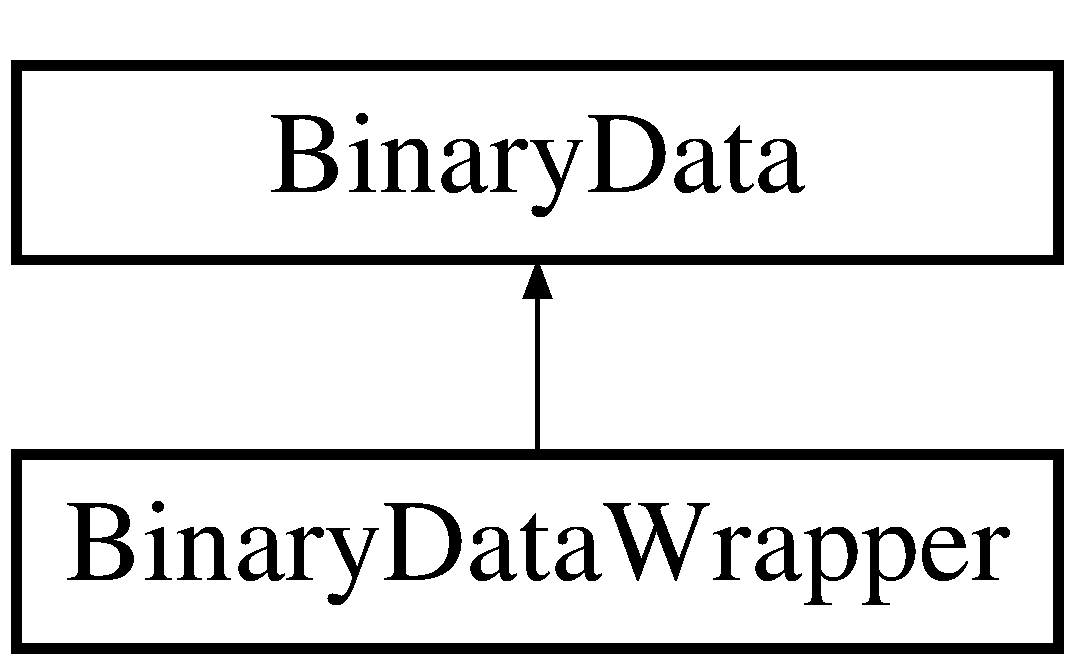
\includegraphics[height=2.000000cm]{dc/d6a/classBinaryDataWrapper}
\end{center}
\end{figure}
\subsection*{Public Member Functions}
\begin{DoxyCompactItemize}
\item 
\hyperlink{classBinaryDataWrapper_a3b8e761eca3c776aa55de4926e9eba8d}{Binary\+Data\+Wrapper} (const std\+::string \&\hyperlink{classBinaryData_a9eae74bdf3b91a3e1461802d820591e3}{file})
\item 
\hyperlink{classBinaryDataWrapper_aab9bf6a3b5a0a267b12bdf65bc44a5de}{$\sim$\+Binary\+Data\+Wrapper} ()
\begin{DoxyCompactList}\small\item\em Empty but needed for unstructured\+Grid destruction. \end{DoxyCompactList}\item 
void \hyperlink{classBinaryDataWrapper_a1cbd933061a05f42ca7ab95cbc951c98}{load\+Result} (\hyperlink{classResult}{Result} \&result, const int \&component)
\begin{DoxyCompactList}\small\item\em Load the given component of the given result, set inner values. \end{DoxyCompactList}\item 
vtk\+Smart\+Pointer$<$ vtk\+Unstructured\+Grid $>$ \hyperlink{classBinaryDataWrapper_a4ab331926387a422e4275f57f37f8f5e}{get\+Unstructured\+Grid} () const
\item 
vtk\+Smart\+Pointer$<$ vtk\+Float\+Array $>$ \hyperlink{classBinaryDataWrapper_a047b8ec79270082144bcb1c990bc4a91}{get\+Scalars} () const
\item 
Q\+String\+List \hyperlink{classBinaryDataWrapper_a7b0d2b52b89c0edf1bfdecf808179efa}{get\+Information\+List} () const
\end{DoxyCompactItemize}
\subsection*{Additional Inherited Members}


\subsection{Detailed Description}
Wrapper around the \hyperlink{classBinaryData}{Binary\+Data} class that allows to interact with V\+TK. 

\subsection{Constructor \& Destructor Documentation}
\mbox{\Hypertarget{classBinaryDataWrapper_a3b8e761eca3c776aa55de4926e9eba8d}\label{classBinaryDataWrapper_a3b8e761eca3c776aa55de4926e9eba8d}} 
\index{Binary\+Data\+Wrapper@{Binary\+Data\+Wrapper}!Binary\+Data\+Wrapper@{Binary\+Data\+Wrapper}}
\index{Binary\+Data\+Wrapper@{Binary\+Data\+Wrapper}!Binary\+Data\+Wrapper@{Binary\+Data\+Wrapper}}
\subsubsection{\texorpdfstring{Binary\+Data\+Wrapper()}{BinaryDataWrapper()}}
{\footnotesize\ttfamily Binary\+Data\+Wrapper\+::\+Binary\+Data\+Wrapper (\begin{DoxyParamCaption}\item[{const std\+::string \&}]{file }\end{DoxyParamCaption})}


\begin{DoxyParams}{Parameters}
{\em file} & Path to the res gz\+File \\
\hline
\end{DoxyParams}
\mbox{\Hypertarget{classBinaryDataWrapper_aab9bf6a3b5a0a267b12bdf65bc44a5de}\label{classBinaryDataWrapper_aab9bf6a3b5a0a267b12bdf65bc44a5de}} 
\index{Binary\+Data\+Wrapper@{Binary\+Data\+Wrapper}!````~Binary\+Data\+Wrapper@{$\sim$\+Binary\+Data\+Wrapper}}
\index{````~Binary\+Data\+Wrapper@{$\sim$\+Binary\+Data\+Wrapper}!Binary\+Data\+Wrapper@{Binary\+Data\+Wrapper}}
\subsubsection{\texorpdfstring{$\sim$\+Binary\+Data\+Wrapper()}{~BinaryDataWrapper()}}
{\footnotesize\ttfamily Binary\+Data\+Wrapper\+::$\sim$\+Binary\+Data\+Wrapper (\begin{DoxyParamCaption}{ }\end{DoxyParamCaption})\hspace{0.3cm}{\ttfamily [default]}}



Empty but needed for unstructured\+Grid destruction. 



\subsection{Member Function Documentation}
\mbox{\Hypertarget{classBinaryDataWrapper_a7b0d2b52b89c0edf1bfdecf808179efa}\label{classBinaryDataWrapper_a7b0d2b52b89c0edf1bfdecf808179efa}} 
\index{Binary\+Data\+Wrapper@{Binary\+Data\+Wrapper}!get\+Information\+List@{get\+Information\+List}}
\index{get\+Information\+List@{get\+Information\+List}!Binary\+Data\+Wrapper@{Binary\+Data\+Wrapper}}
\subsubsection{\texorpdfstring{get\+Information\+List()}{getInformationList()}}
{\footnotesize\ttfamily Q\+String\+List Binary\+Data\+Wrapper\+::get\+Information\+List (\begin{DoxyParamCaption}{ }\end{DoxyParamCaption}) const}

\begin{DoxyReturn}{Returns}
Information about the current results as a QT usable object 
\end{DoxyReturn}
\mbox{\Hypertarget{classBinaryDataWrapper_a047b8ec79270082144bcb1c990bc4a91}\label{classBinaryDataWrapper_a047b8ec79270082144bcb1c990bc4a91}} 
\index{Binary\+Data\+Wrapper@{Binary\+Data\+Wrapper}!get\+Scalars@{get\+Scalars}}
\index{get\+Scalars@{get\+Scalars}!Binary\+Data\+Wrapper@{Binary\+Data\+Wrapper}}
\subsubsection{\texorpdfstring{get\+Scalars()}{getScalars()}}
{\footnotesize\ttfamily vtk\+Smart\+Pointer$<$ vtk\+Float\+Array $>$ Binary\+Data\+Wrapper\+::get\+Scalars (\begin{DoxyParamCaption}{ }\end{DoxyParamCaption}) const}

\begin{DoxyReturn}{Returns}
Observed values of the loaded result 
\end{DoxyReturn}
\mbox{\Hypertarget{classBinaryDataWrapper_a4ab331926387a422e4275f57f37f8f5e}\label{classBinaryDataWrapper_a4ab331926387a422e4275f57f37f8f5e}} 
\index{Binary\+Data\+Wrapper@{Binary\+Data\+Wrapper}!get\+Unstructured\+Grid@{get\+Unstructured\+Grid}}
\index{get\+Unstructured\+Grid@{get\+Unstructured\+Grid}!Binary\+Data\+Wrapper@{Binary\+Data\+Wrapper}}
\subsubsection{\texorpdfstring{get\+Unstructured\+Grid()}{getUnstructuredGrid()}}
{\footnotesize\ttfamily vtk\+Smart\+Pointer$<$ vtk\+Unstructured\+Grid $>$ Binary\+Data\+Wrapper\+::get\+Unstructured\+Grid (\begin{DoxyParamCaption}{ }\end{DoxyParamCaption}) const}

\begin{DoxyReturn}{Returns}
The Data\+Set of points of the loaded and converted GiD resource file 
\end{DoxyReturn}
\mbox{\Hypertarget{classBinaryDataWrapper_a1cbd933061a05f42ca7ab95cbc951c98}\label{classBinaryDataWrapper_a1cbd933061a05f42ca7ab95cbc951c98}} 
\index{Binary\+Data\+Wrapper@{Binary\+Data\+Wrapper}!load\+Result@{load\+Result}}
\index{load\+Result@{load\+Result}!Binary\+Data\+Wrapper@{Binary\+Data\+Wrapper}}
\subsubsection{\texorpdfstring{load\+Result()}{loadResult()}}
{\footnotesize\ttfamily void Binary\+Data\+Wrapper\+::load\+Result (\begin{DoxyParamCaption}\item[{\hyperlink{classResult}{Result} \&}]{result,  }\item[{const int \&}]{component }\end{DoxyParamCaption})}



Load the given component of the given result, set inner values. 


\begin{DoxyParams}{Parameters}
{\em result} & \hyperlink{classResult}{Result} to load \\
\hline
{\em component} & Component to load \\
\hline
\end{DoxyParams}


The documentation for this class was generated from the following files\+:\begin{DoxyCompactItemize}
\item 
include/\hyperlink{binary__data__wrapper_8h}{binary\+\_\+data\+\_\+wrapper.\+h}\item 
src/\hyperlink{binary__data__wrapper_8cpp}{binary\+\_\+data\+\_\+wrapper.\+cpp}\end{DoxyCompactItemize}

\hypertarget{classMainWindow}{}\section{Main\+Window Class Reference}
\label{classMainWindow}\index{Main\+Window@{Main\+Window}}


Qt main window.  




{\ttfamily \#include $<$main\+\_\+window.\+h$>$}

Inheritance diagram for Main\+Window\+:\begin{figure}[H]
\begin{center}
\leavevmode
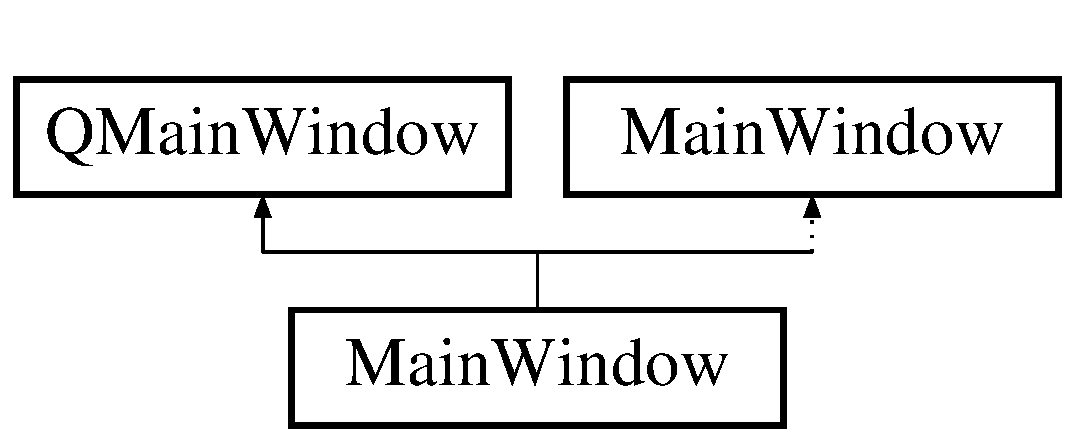
\includegraphics[height=2.000000cm]{d6/d1a/classMainWindow}
\end{center}
\end{figure}
\subsection*{Public Slots}
\begin{DoxyCompactItemize}
\item 
void \hyperlink{classMainWindow_aca3b7226e638a0cd5ef9d7db749ff67e}{slot\+Exit} ()
\item 
void \hyperlink{classMainWindow_a2ef511727fce3fc9bdf17a73f078cec7}{slot\+Open\+File} ()
\item 
void \hyperlink{classMainWindow_a73d6c706bae3e712ab654a78d1921c89}{slot\+Reset\+Camera} ()
\item 
void \hyperlink{classMainWindow_ab4be74f01161ac57ddf86f32c60137d3}{slot\+Zoom\+Area} ()
\item 
void \hyperlink{classMainWindow_ab2c27d510eabe77a0eb11fc091adc293}{slot\+Interact\+With\+Object} ()
\item 
void \hyperlink{classMainWindow_a914c794d921ccfcd861284bc8cd9f96a}{slot\+Result} (\hyperlink{classResult}{Result} \&result, const unsigned int \&component)
\end{DoxyCompactItemize}
\subsection*{Public Member Functions}
\begin{DoxyCompactItemize}
\item 
\hyperlink{classMainWindow_a06c3eabf20b0ef52c0b33208334e8e1f}{Main\+Window} (char $\ast$data\+Directory)
\end{DoxyCompactItemize}


\subsection{Detailed Description}
Qt main window. 

\subsection{Constructor \& Destructor Documentation}
\mbox{\Hypertarget{classMainWindow_a06c3eabf20b0ef52c0b33208334e8e1f}\label{classMainWindow_a06c3eabf20b0ef52c0b33208334e8e1f}} 
\index{Main\+Window@{Main\+Window}!Main\+Window@{Main\+Window}}
\index{Main\+Window@{Main\+Window}!Main\+Window@{Main\+Window}}
\subsubsection{\texorpdfstring{Main\+Window()}{MainWindow()}}
{\footnotesize\ttfamily Main\+Window\+::\+Main\+Window (\begin{DoxyParamCaption}\item[{char $\ast$}]{data\+Directory }\end{DoxyParamCaption})}


\begin{DoxyParams}{Parameters}
{\em data\+Directory} & The path to the objects directory \\
\hline
\end{DoxyParams}


\subsection{Member Function Documentation}
\mbox{\Hypertarget{classMainWindow_aca3b7226e638a0cd5ef9d7db749ff67e}\label{classMainWindow_aca3b7226e638a0cd5ef9d7db749ff67e}} 
\index{Main\+Window@{Main\+Window}!slot\+Exit@{slot\+Exit}}
\index{slot\+Exit@{slot\+Exit}!Main\+Window@{Main\+Window}}
\subsubsection{\texorpdfstring{slot\+Exit}{slotExit}}
{\footnotesize\ttfamily void Main\+Window\+::slot\+Exit (\begin{DoxyParamCaption}{ }\end{DoxyParamCaption})\hspace{0.3cm}{\ttfamily [slot]}}

Stop the application \mbox{\Hypertarget{classMainWindow_ab2c27d510eabe77a0eb11fc091adc293}\label{classMainWindow_ab2c27d510eabe77a0eb11fc091adc293}} 
\index{Main\+Window@{Main\+Window}!slot\+Interact\+With\+Object@{slot\+Interact\+With\+Object}}
\index{slot\+Interact\+With\+Object@{slot\+Interact\+With\+Object}!Main\+Window@{Main\+Window}}
\subsubsection{\texorpdfstring{slot\+Interact\+With\+Object}{slotInteractWithObject}}
{\footnotesize\ttfamily void Main\+Window\+::slot\+Interact\+With\+Object (\begin{DoxyParamCaption}{ }\end{DoxyParamCaption})\hspace{0.3cm}{\ttfamily [slot]}}

Reset the interactor to allow object interaction after zoom\+Area \mbox{\Hypertarget{classMainWindow_a2ef511727fce3fc9bdf17a73f078cec7}\label{classMainWindow_a2ef511727fce3fc9bdf17a73f078cec7}} 
\index{Main\+Window@{Main\+Window}!slot\+Open\+File@{slot\+Open\+File}}
\index{slot\+Open\+File@{slot\+Open\+File}!Main\+Window@{Main\+Window}}
\subsubsection{\texorpdfstring{slot\+Open\+File}{slotOpenFile}}
{\footnotesize\ttfamily void Main\+Window\+::slot\+Open\+File (\begin{DoxyParamCaption}{ }\end{DoxyParamCaption})\hspace{0.3cm}{\ttfamily [slot]}}

Open and read object file, then render it \mbox{\Hypertarget{classMainWindow_a73d6c706bae3e712ab654a78d1921c89}\label{classMainWindow_a73d6c706bae3e712ab654a78d1921c89}} 
\index{Main\+Window@{Main\+Window}!slot\+Reset\+Camera@{slot\+Reset\+Camera}}
\index{slot\+Reset\+Camera@{slot\+Reset\+Camera}!Main\+Window@{Main\+Window}}
\subsubsection{\texorpdfstring{slot\+Reset\+Camera}{slotResetCamera}}
{\footnotesize\ttfamily void Main\+Window\+::slot\+Reset\+Camera (\begin{DoxyParamCaption}{ }\end{DoxyParamCaption})\hspace{0.3cm}{\ttfamily [slot]}}

Reset the camera view as default \mbox{\Hypertarget{classMainWindow_a914c794d921ccfcd861284bc8cd9f96a}\label{classMainWindow_a914c794d921ccfcd861284bc8cd9f96a}} 
\index{Main\+Window@{Main\+Window}!slot\+Result@{slot\+Result}}
\index{slot\+Result@{slot\+Result}!Main\+Window@{Main\+Window}}
\subsubsection{\texorpdfstring{slot\+Result}{slotResult}}
{\footnotesize\ttfamily void Main\+Window\+::slot\+Result (\begin{DoxyParamCaption}\item[{\hyperlink{classResult}{Result} \&}]{result,  }\item[{const unsigned int \&}]{component }\end{DoxyParamCaption})\hspace{0.3cm}{\ttfamily [slot]}}

Select the result to visualise 
\begin{DoxyParams}{Parameters}
{\em result} & \hyperlink{classResult}{Result} to visualise \\
\hline
{\em component} & Choice for set\+V\+TK method \\
\hline
\end{DoxyParams}
\mbox{\Hypertarget{classMainWindow_ab4be74f01161ac57ddf86f32c60137d3}\label{classMainWindow_ab4be74f01161ac57ddf86f32c60137d3}} 
\index{Main\+Window@{Main\+Window}!slot\+Zoom\+Area@{slot\+Zoom\+Area}}
\index{slot\+Zoom\+Area@{slot\+Zoom\+Area}!Main\+Window@{Main\+Window}}
\subsubsection{\texorpdfstring{slot\+Zoom\+Area}{slotZoomArea}}
{\footnotesize\ttfamily void Main\+Window\+::slot\+Zoom\+Area (\begin{DoxyParamCaption}{ }\end{DoxyParamCaption})\hspace{0.3cm}{\ttfamily [slot]}}

Allow the user to select an area to zoom on 

The documentation for this class was generated from the following files\+:\begin{DoxyCompactItemize}
\item 
include/\hyperlink{main__window_8h}{main\+\_\+window.\+h}\item 
src/\hyperlink{main__window_8cpp}{main\+\_\+window.\+cpp}\end{DoxyCompactItemize}

\hypertarget{classMesh}{}\section{Mesh Class Reference}
\label{classMesh}\index{Mesh@{Mesh}}


Representation of a mesh, all of its nodes and elements.  




{\ttfamily \#include $<$mesh.\+h$>$}

\subsection*{Public Member Functions}
\begin{DoxyCompactItemize}
\item 
\hyperlink{classMesh_a7648013c55e45a4cde14d75b14631751}{Mesh} (gz\+File file, \hyperlink{utilities_8h_a981a882ef2a0d7ee5b6b32f27105644e}{data\+Fields} fields)
\item 
std\+::string \hyperlink{classMesh_a7582c53a358e1f5f85c745e8845b45a2}{get\+Name} ()
\item 
std\+::string \hyperlink{classMesh_a59688b2769be829f3142662d5dec4855}{get\+Element\+Name} ()
\item 
Gi\+D\+\_\+\+Element\+Type \hyperlink{classMesh_aafbb679e494fcebacd811384bc3d9e29}{get\+Element\+Type} ()
\item 
unsigned int \hyperlink{classMesh_aded45a45edb90ce60215df2f69fdedac}{get\+Dim\+Count} () const
\item 
unsigned int \hyperlink{classMesh_a89191e32a7f1ab3206bc9ea88be42dda}{get\+Node\+Count} () const
\item 
unsigned int \hyperlink{classMesh_a9d0881d1942c4a0b8d08a4f440f1c3ea}{get\+Element\+Count} () const
\item 
std\+::vector$<$ \hyperlink{classNode}{Node} $>$ \hyperlink{classMesh_a9daa8d1054eabf200d152bba156a2ebe}{get\+Nodes} ()
\item 
std\+::tuple$<$ int \&, int $\ast$ $>$ \hyperlink{classMesh_a415ffa23e4dcb0c73b60557455e87b25}{get\+Element} (const unsigned int \&id) const
\end{DoxyCompactItemize}
\subsection*{Static Public Member Functions}
\begin{DoxyCompactItemize}
\item 
static Gi\+D\+\_\+\+Element\+Type \hyperlink{classMesh_aec161b91369a8f24ce2fa333547a7eef}{get\+Gi\+D\+Element\+Type} (const char $\ast$element)
\begin{DoxyCompactList}\small\item\em Write the mesh into a currently open Post\+Result\+File. \end{DoxyCompactList}\end{DoxyCompactItemize}
\subsection*{Static Public Attributes}
\begin{DoxyCompactItemize}
\item 
static size\+\_\+t \hyperlink{classMesh_aba7b72605589dfd0a54bf5fa945774b3}{max\+Node\+Count} = 0
\begin{DoxyCompactList}\small\item\em Biggest number of node encountered in the mesh. \end{DoxyCompactList}\item 
static const std\+::map$<$ std\+::string, Gi\+D\+\_\+\+Element\+Type $>$ \hyperlink{classMesh_a05bb4cbffc09e209148c384a1f84aa9a}{Gi\+D\+\_\+\+Element\+Type\+Encoding}
\begin{DoxyCompactList}\small\item\em Map of all recognized Gi\+D\+\_\+\+Element\+Type according to their string encoded value. \end{DoxyCompactList}\end{DoxyCompactItemize}


\subsection{Detailed Description}
Representation of a mesh, all of its nodes and elements. 

\subsection{Constructor \& Destructor Documentation}
\mbox{\Hypertarget{classMesh_a7648013c55e45a4cde14d75b14631751}\label{classMesh_a7648013c55e45a4cde14d75b14631751}} 
\index{Mesh@{Mesh}!Mesh@{Mesh}}
\index{Mesh@{Mesh}!Mesh@{Mesh}}
\subsubsection{\texorpdfstring{Mesh()}{Mesh()}}
{\footnotesize\ttfamily Mesh\+::\+Mesh (\begin{DoxyParamCaption}\item[{gz\+File}]{file,  }\item[{\hyperlink{utilities_8h_a981a882ef2a0d7ee5b6b32f27105644e}{data\+Fields}}]{fields }\end{DoxyParamCaption})}


\begin{DoxyParams}{Parameters}
{\em file} & File that contains the mesh information \\
\hline
{\em fields} & Base fields read from the file \\
\hline
\end{DoxyParams}


\subsection{Member Function Documentation}
\mbox{\Hypertarget{classMesh_aded45a45edb90ce60215df2f69fdedac}\label{classMesh_aded45a45edb90ce60215df2f69fdedac}} 
\index{Mesh@{Mesh}!get\+Dim\+Count@{get\+Dim\+Count}}
\index{get\+Dim\+Count@{get\+Dim\+Count}!Mesh@{Mesh}}
\subsubsection{\texorpdfstring{get\+Dim\+Count()}{getDimCount()}}
{\footnotesize\ttfamily unsigned int Mesh\+::get\+Dim\+Count (\begin{DoxyParamCaption}{ }\end{DoxyParamCaption}) const}

\begin{DoxyReturn}{Returns}
The number of dimension of the mesh (2 or 3) 
\end{DoxyReturn}
\mbox{\Hypertarget{classMesh_a415ffa23e4dcb0c73b60557455e87b25}\label{classMesh_a415ffa23e4dcb0c73b60557455e87b25}} 
\index{Mesh@{Mesh}!get\+Element@{get\+Element}}
\index{get\+Element@{get\+Element}!Mesh@{Mesh}}
\subsubsection{\texorpdfstring{get\+Element()}{getElement()}}
{\footnotesize\ttfamily std\+::tuple$<$ int \&, int $\ast$ $>$ Mesh\+::get\+Element (\begin{DoxyParamCaption}\item[{const unsigned int \&}]{id }\end{DoxyParamCaption}) const}


\begin{DoxyParams}{Parameters}
{\em id} & ID of the element \\
\hline
\end{DoxyParams}
\begin{DoxyReturn}{Returns}
Return information about an element\+: 
\end{DoxyReturn}
\mbox{\Hypertarget{classMesh_a9d0881d1942c4a0b8d08a4f440f1c3ea}\label{classMesh_a9d0881d1942c4a0b8d08a4f440f1c3ea}} 
\index{Mesh@{Mesh}!get\+Element\+Count@{get\+Element\+Count}}
\index{get\+Element\+Count@{get\+Element\+Count}!Mesh@{Mesh}}
\subsubsection{\texorpdfstring{get\+Element\+Count()}{getElementCount()}}
{\footnotesize\ttfamily unsigned int Mesh\+::get\+Element\+Count (\begin{DoxyParamCaption}{ }\end{DoxyParamCaption}) const}

\begin{DoxyReturn}{Returns}
The number of elements in the mesh 
\end{DoxyReturn}
\mbox{\Hypertarget{classMesh_a59688b2769be829f3142662d5dec4855}\label{classMesh_a59688b2769be829f3142662d5dec4855}} 
\index{Mesh@{Mesh}!get\+Element\+Name@{get\+Element\+Name}}
\index{get\+Element\+Name@{get\+Element\+Name}!Mesh@{Mesh}}
\subsubsection{\texorpdfstring{get\+Element\+Name()}{getElementName()}}
{\footnotesize\ttfamily std\+::string Mesh\+::get\+Element\+Name (\begin{DoxyParamCaption}{ }\end{DoxyParamCaption})}

\begin{DoxyReturn}{Returns}
The string encoded element type of the mesh 
\end{DoxyReturn}
\mbox{\Hypertarget{classMesh_aafbb679e494fcebacd811384bc3d9e29}\label{classMesh_aafbb679e494fcebacd811384bc3d9e29}} 
\index{Mesh@{Mesh}!get\+Element\+Type@{get\+Element\+Type}}
\index{get\+Element\+Type@{get\+Element\+Type}!Mesh@{Mesh}}
\subsubsection{\texorpdfstring{get\+Element\+Type()}{getElementType()}}
{\footnotesize\ttfamily Gi\+D\+\_\+\+Element\+Type Mesh\+::get\+Element\+Type (\begin{DoxyParamCaption}{ }\end{DoxyParamCaption})}

\begin{DoxyReturn}{Returns}
The Element type of the mesh 
\end{DoxyReturn}
\mbox{\Hypertarget{classMesh_aec161b91369a8f24ce2fa333547a7eef}\label{classMesh_aec161b91369a8f24ce2fa333547a7eef}} 
\index{Mesh@{Mesh}!get\+Gi\+D\+Element\+Type@{get\+Gi\+D\+Element\+Type}}
\index{get\+Gi\+D\+Element\+Type@{get\+Gi\+D\+Element\+Type}!Mesh@{Mesh}}
\subsubsection{\texorpdfstring{get\+Gi\+D\+Element\+Type()}{getGiDElementType()}}
{\footnotesize\ttfamily Gi\+D\+\_\+\+Element\+Type Mesh\+::get\+Gi\+D\+Element\+Type (\begin{DoxyParamCaption}\item[{const char $\ast$}]{element }\end{DoxyParamCaption})\hspace{0.3cm}{\ttfamily [static]}}



Write the mesh into a currently open Post\+Result\+File. 

\begin{DoxyReturn}{Returns}
The state of the GiD Post \hyperlink{classMesh}{Mesh} closure Get the Gi\+D\+\_\+\+Element\+Type of a string encoded Gi\+D\+Element\+Type 
\end{DoxyReturn}

\begin{DoxyParams}{Parameters}
{\em element} & string encoded Gi\+D\+\_\+\+Element\+Type \\
\hline
\end{DoxyParams}
\begin{DoxyReturn}{Returns}
The according Gi\+D\+\_\+\+Element\+Type, Gi\+D\+\_\+\+No\+Element by default 
\end{DoxyReturn}

\begin{DoxyExceptions}{Exceptions}
{\em runtime\+\_\+error} & if the encoded Gi\+D\+\_\+\+Element\+Type is not recognized \\
\hline
\end{DoxyExceptions}
\mbox{\Hypertarget{classMesh_a7582c53a358e1f5f85c745e8845b45a2}\label{classMesh_a7582c53a358e1f5f85c745e8845b45a2}} 
\index{Mesh@{Mesh}!get\+Name@{get\+Name}}
\index{get\+Name@{get\+Name}!Mesh@{Mesh}}
\subsubsection{\texorpdfstring{get\+Name()}{getName()}}
{\footnotesize\ttfamily std\+::string Mesh\+::get\+Name (\begin{DoxyParamCaption}{ }\end{DoxyParamCaption})}

\begin{DoxyReturn}{Returns}
The name of the name 
\end{DoxyReturn}
\mbox{\Hypertarget{classMesh_a89191e32a7f1ab3206bc9ea88be42dda}\label{classMesh_a89191e32a7f1ab3206bc9ea88be42dda}} 
\index{Mesh@{Mesh}!get\+Node\+Count@{get\+Node\+Count}}
\index{get\+Node\+Count@{get\+Node\+Count}!Mesh@{Mesh}}
\subsubsection{\texorpdfstring{get\+Node\+Count()}{getNodeCount()}}
{\footnotesize\ttfamily unsigned int Mesh\+::get\+Node\+Count (\begin{DoxyParamCaption}{ }\end{DoxyParamCaption}) const}

\begin{DoxyReturn}{Returns}
The number of nodes that constitutes the mesh 
\end{DoxyReturn}
\mbox{\Hypertarget{classMesh_a9daa8d1054eabf200d152bba156a2ebe}\label{classMesh_a9daa8d1054eabf200d152bba156a2ebe}} 
\index{Mesh@{Mesh}!get\+Nodes@{get\+Nodes}}
\index{get\+Nodes@{get\+Nodes}!Mesh@{Mesh}}
\subsubsection{\texorpdfstring{get\+Nodes()}{getNodes()}}
{\footnotesize\ttfamily std\+::vector$<$\hyperlink{classNode}{Node}$>$ Mesh\+::get\+Nodes (\begin{DoxyParamCaption}{ }\end{DoxyParamCaption})}

\begin{DoxyReturn}{Returns}
The nodes that constitutes the mesh 
\end{DoxyReturn}


\subsection{Member Data Documentation}
\mbox{\Hypertarget{classMesh_a05bb4cbffc09e209148c384a1f84aa9a}\label{classMesh_a05bb4cbffc09e209148c384a1f84aa9a}} 
\index{Mesh@{Mesh}!Gi\+D\+\_\+\+Element\+Type\+Encoding@{Gi\+D\+\_\+\+Element\+Type\+Encoding}}
\index{Gi\+D\+\_\+\+Element\+Type\+Encoding@{Gi\+D\+\_\+\+Element\+Type\+Encoding}!Mesh@{Mesh}}
\subsubsection{\texorpdfstring{Gi\+D\+\_\+\+Element\+Type\+Encoding}{GiD\_ElementTypeEncoding}}
{\footnotesize\ttfamily const std\+::map$<$ std\+::string, Gi\+D\+\_\+\+Element\+Type $>$ Mesh\+::\+Gi\+D\+\_\+\+Element\+Type\+Encoding\hspace{0.3cm}{\ttfamily [static]}}

{\bfseries Initial value\+:}
\begin{DoxyCode}
= \{
    \{ \textcolor{stringliteral}{""}, GiD\_NoElement \},
    \{ \textcolor{stringliteral}{"Point"}, GiD\_NoElement \},
    \{ \textcolor{stringliteral}{"Linear"}, GiD\_NoElement \},
    \{ \textcolor{stringliteral}{"Triangle"}, GiD\_Triangle \},
    \{ \textcolor{stringliteral}{"Quadrilateral"}, GiD\_Quadrilateral \},
    \{ \textcolor{stringliteral}{"Tetrahedra"}, GiD\_Tetrahedra \},
    \{ \textcolor{stringliteral}{"Hexahedra"}, GiD\_Hexahedra \},
    \{ \textcolor{stringliteral}{"Prism"}, GiD\_Prism \},
    \{ \textcolor{stringliteral}{"Pyramid"}, GiD\_NoElement \},
    \{ \textcolor{stringliteral}{"Sphere"}, GiD\_NoElement \},
    \{ \textcolor{stringliteral}{"Circle"}, GiD\_NoElement \}
\}
\end{DoxyCode}


Map of all recognized Gi\+D\+\_\+\+Element\+Type according to their string encoded value. 

\mbox{\Hypertarget{classMesh_aba7b72605589dfd0a54bf5fa945774b3}\label{classMesh_aba7b72605589dfd0a54bf5fa945774b3}} 
\index{Mesh@{Mesh}!max\+Node\+Count@{max\+Node\+Count}}
\index{max\+Node\+Count@{max\+Node\+Count}!Mesh@{Mesh}}
\subsubsection{\texorpdfstring{max\+Node\+Count}{maxNodeCount}}
{\footnotesize\ttfamily size\+\_\+t Mesh\+::max\+Node\+Count = 0\hspace{0.3cm}{\ttfamily [static]}}



Biggest number of node encountered in the mesh. 



The documentation for this class was generated from the following files\+:\begin{DoxyCompactItemize}
\item 
include/\hyperlink{mesh_8h}{mesh.\+h}\item 
src/\hyperlink{mesh_8cpp}{mesh.\+cpp}\end{DoxyCompactItemize}

\hypertarget{classNode}{}\section{Node Class Reference}
\label{classNode}\index{Node@{Node}}


Point in 3D space representation, part of a \hyperlink{classMesh}{Mesh}.  




{\ttfamily \#include $<$mesh.\+h$>$}

\subsection*{Public Member Functions}
\begin{DoxyCompactItemize}
\item 
\hyperlink{classNode_a232677901f5187ef510360008d8cf3e0}{Node} (unsigned int id, const float $\ast$coord)
\item 
\hyperlink{classNode_acf01ac83ce5412472a26220fe1cdc748}{Node} (unsigned int id, float x, float y, float z)
\item 
unsigned int \hyperlink{classNode_af9b4c1c72ce14b69f5e99deb4440f489}{get\+Id} () const
\item 
const float $\ast$ \hyperlink{classNode_ad1fb25b09446913847578ab0b8de6cdb}{get\+Coords} ()
\item 
float \hyperlink{classNode_a98ba03ab2272a479d3173932a40c3a41}{getX} ()
\item 
float \hyperlink{classNode_a55366d94e5244071158b45b31c43dd8b}{getY} ()
\item 
float \hyperlink{classNode_ad275f03c5bf56c9ec572ff1da10bb34c}{getZ} ()
\end{DoxyCompactItemize}


\subsection{Detailed Description}
Point in 3D space representation, part of a \hyperlink{classMesh}{Mesh}. 

\begin{DoxySeeAlso}{See also}
\hyperlink{classMesh}{Mesh} 
\end{DoxySeeAlso}


\subsection{Constructor \& Destructor Documentation}
\mbox{\Hypertarget{classNode_a232677901f5187ef510360008d8cf3e0}\label{classNode_a232677901f5187ef510360008d8cf3e0}} 
\index{Node@{Node}!Node@{Node}}
\index{Node@{Node}!Node@{Node}}
\subsubsection{\texorpdfstring{Node()}{Node()}\hspace{0.1cm}{\footnotesize\ttfamily [1/2]}}
{\footnotesize\ttfamily Node\+::\+Node (\begin{DoxyParamCaption}\item[{unsigned int}]{id,  }\item[{const float $\ast$}]{coord }\end{DoxyParamCaption})}


\begin{DoxyParams}{Parameters}
{\em id} & ID of the current \hyperlink{classNode}{Node} \\
\hline
{\em coord} & Space coordinates of the node \\
\hline
\end{DoxyParams}
\mbox{\Hypertarget{classNode_acf01ac83ce5412472a26220fe1cdc748}\label{classNode_acf01ac83ce5412472a26220fe1cdc748}} 
\index{Node@{Node}!Node@{Node}}
\index{Node@{Node}!Node@{Node}}
\subsubsection{\texorpdfstring{Node()}{Node()}\hspace{0.1cm}{\footnotesize\ttfamily [2/2]}}
{\footnotesize\ttfamily Node\+::\+Node (\begin{DoxyParamCaption}\item[{unsigned int}]{id,  }\item[{float}]{x,  }\item[{float}]{y,  }\item[{float}]{z }\end{DoxyParamCaption})}


\begin{DoxyParams}{Parameters}
{\em id} & ID of the current \hyperlink{classNode}{Node} \\
\hline
{\em x} & X component of the Space coordinates of the node \\
\hline
{\em y} & Y component of the Space coordinates of the node \\
\hline
{\em z} & Z component of the Space coordinates of the node \\
\hline
\end{DoxyParams}


\subsection{Member Function Documentation}
\mbox{\Hypertarget{classNode_ad1fb25b09446913847578ab0b8de6cdb}\label{classNode_ad1fb25b09446913847578ab0b8de6cdb}} 
\index{Node@{Node}!get\+Coords@{get\+Coords}}
\index{get\+Coords@{get\+Coords}!Node@{Node}}
\subsubsection{\texorpdfstring{get\+Coords()}{getCoords()}}
{\footnotesize\ttfamily const float $\ast$ Node\+::get\+Coords (\begin{DoxyParamCaption}{ }\end{DoxyParamCaption})}

\begin{DoxyReturn}{Returns}
The pointer of the space coordinates of the node 
\end{DoxyReturn}
\mbox{\Hypertarget{classNode_af9b4c1c72ce14b69f5e99deb4440f489}\label{classNode_af9b4c1c72ce14b69f5e99deb4440f489}} 
\index{Node@{Node}!get\+Id@{get\+Id}}
\index{get\+Id@{get\+Id}!Node@{Node}}
\subsubsection{\texorpdfstring{get\+Id()}{getId()}}
{\footnotesize\ttfamily unsigned int Node\+::get\+Id (\begin{DoxyParamCaption}{ }\end{DoxyParamCaption}) const}

\begin{DoxyReturn}{Returns}
The ID of the node 
\end{DoxyReturn}
\mbox{\Hypertarget{classNode_a98ba03ab2272a479d3173932a40c3a41}\label{classNode_a98ba03ab2272a479d3173932a40c3a41}} 
\index{Node@{Node}!getX@{getX}}
\index{getX@{getX}!Node@{Node}}
\subsubsection{\texorpdfstring{get\+X()}{getX()}}
{\footnotesize\ttfamily float Node\+::getX (\begin{DoxyParamCaption}{ }\end{DoxyParamCaption})}

\begin{DoxyReturn}{Returns}
The X space coordinates component of the node 
\end{DoxyReturn}
\mbox{\Hypertarget{classNode_a55366d94e5244071158b45b31c43dd8b}\label{classNode_a55366d94e5244071158b45b31c43dd8b}} 
\index{Node@{Node}!getY@{getY}}
\index{getY@{getY}!Node@{Node}}
\subsubsection{\texorpdfstring{get\+Y()}{getY()}}
{\footnotesize\ttfamily float Node\+::getY (\begin{DoxyParamCaption}{ }\end{DoxyParamCaption})}

\begin{DoxyReturn}{Returns}
The Y space coordinates component of the node 
\end{DoxyReturn}
\mbox{\Hypertarget{classNode_ad275f03c5bf56c9ec572ff1da10bb34c}\label{classNode_ad275f03c5bf56c9ec572ff1da10bb34c}} 
\index{Node@{Node}!getZ@{getZ}}
\index{getZ@{getZ}!Node@{Node}}
\subsubsection{\texorpdfstring{get\+Z()}{getZ()}}
{\footnotesize\ttfamily float Node\+::getZ (\begin{DoxyParamCaption}{ }\end{DoxyParamCaption})}

\begin{DoxyReturn}{Returns}
The Z space coordinates component of the node 
\end{DoxyReturn}


The documentation for this class was generated from the following files\+:\begin{DoxyCompactItemize}
\item 
include/\hyperlink{mesh_8h}{mesh.\+h}\item 
src/\hyperlink{mesh_8cpp}{mesh.\+cpp}\end{DoxyCompactItemize}

\hypertarget{classResult}{}\section{Result Class Reference}
\label{classResult}\index{Result@{Result}}


Representation of all the results and their components read from a res file.  




{\ttfamily \#include $<$result.\+h$>$}

\subsection*{Public Member Functions}
\begin{DoxyCompactItemize}
\item 
\hyperlink{classResult_aebbe4a0e66acff6edd381f2a6c7c46df}{Result} (gz\+File file, \hyperlink{utilities_8h_a981a882ef2a0d7ee5b6b32f27105644e}{data\+Fields} fields, int component\+Count)
\item 
std\+::string \hyperlink{classResult_ae9109a2e288a93e1c08d1e495f59191f}{get\+Analysis} ()
\item 
std\+::string \hyperlink{classResult_ad7d2789c7ec7187c67ef1541bd59f214}{get\+Result\+Type} ()
\item 
float \hyperlink{classResult_ae152b587e08f50380c6fc0a54faa08c5}{get\+Step} () const
\item 
int \hyperlink{classResult_a3385ff986211d42ed68d917f365413b9}{get\+Component\+Count} () const
\item 
unsigned int \hyperlink{classResult_a13c7c3058d5d8e2b52a31091061199d3}{get\+Values\+Count} () const
\item 
std\+::vector$<$ std\+::string $>$ \hyperlink{classResult_a20f951753ffd91535a66ec365e2256ff}{get\+Components} ()
\item 
std\+::tuple$<$ int \&, float $\ast$ $>$ \hyperlink{classResult_a987118e44f4275e394a27519fa9c70b1}{get\+Result} (const unsigned int \&id)
\end{DoxyCompactItemize}


\subsection{Detailed Description}
Representation of all the results and their components read from a res file. 

\subsection{Constructor \& Destructor Documentation}
\mbox{\Hypertarget{classResult_aebbe4a0e66acff6edd381f2a6c7c46df}\label{classResult_aebbe4a0e66acff6edd381f2a6c7c46df}} 
\index{Result@{Result}!Result@{Result}}
\index{Result@{Result}!Result@{Result}}
\subsubsection{\texorpdfstring{Result()}{Result()}}
{\footnotesize\ttfamily Result\+::\+Result (\begin{DoxyParamCaption}\item[{gz\+File}]{file,  }\item[{\hyperlink{utilities_8h_a981a882ef2a0d7ee5b6b32f27105644e}{data\+Fields}}]{fields,  }\item[{int}]{component\+Count }\end{DoxyParamCaption})}


\begin{DoxyParams}{Parameters}
{\em file} & res gz\+File \\
\hline
{\em fields} & Base fields read from the file \\
\hline
{\em component\+Count} & Number of component to seek into the result data \\
\hline
\end{DoxyParams}


\subsection{Member Function Documentation}
\mbox{\Hypertarget{classResult_ae9109a2e288a93e1c08d1e495f59191f}\label{classResult_ae9109a2e288a93e1c08d1e495f59191f}} 
\index{Result@{Result}!get\+Analysis@{get\+Analysis}}
\index{get\+Analysis@{get\+Analysis}!Result@{Result}}
\subsubsection{\texorpdfstring{get\+Analysis()}{getAnalysis()}}
{\footnotesize\ttfamily std\+::string Result\+::get\+Analysis (\begin{DoxyParamCaption}{ }\end{DoxyParamCaption})}

\begin{DoxyReturn}{Returns}
The type of analysis of the result 
\end{DoxyReturn}
\mbox{\Hypertarget{classResult_a3385ff986211d42ed68d917f365413b9}\label{classResult_a3385ff986211d42ed68d917f365413b9}} 
\index{Result@{Result}!get\+Component\+Count@{get\+Component\+Count}}
\index{get\+Component\+Count@{get\+Component\+Count}!Result@{Result}}
\subsubsection{\texorpdfstring{get\+Component\+Count()}{getComponentCount()}}
{\footnotesize\ttfamily int Result\+::get\+Component\+Count (\begin{DoxyParamCaption}{ }\end{DoxyParamCaption}) const}

\begin{DoxyReturn}{Returns}
The number component of the result (1 or 4) 
\end{DoxyReturn}
\mbox{\Hypertarget{classResult_a20f951753ffd91535a66ec365e2256ff}\label{classResult_a20f951753ffd91535a66ec365e2256ff}} 
\index{Result@{Result}!get\+Components@{get\+Components}}
\index{get\+Components@{get\+Components}!Result@{Result}}
\subsubsection{\texorpdfstring{get\+Components()}{getComponents()}}
{\footnotesize\ttfamily std\+::vector$<$ std\+::string $>$ Result\+::get\+Components (\begin{DoxyParamCaption}{ }\end{DoxyParamCaption})}

\begin{DoxyReturn}{Returns}
The components of the result (X, Y, Z, M) 
\end{DoxyReturn}
\mbox{\Hypertarget{classResult_a987118e44f4275e394a27519fa9c70b1}\label{classResult_a987118e44f4275e394a27519fa9c70b1}} 
\index{Result@{Result}!get\+Result@{get\+Result}}
\index{get\+Result@{get\+Result}!Result@{Result}}
\subsubsection{\texorpdfstring{get\+Result()}{getResult()}}
{\footnotesize\ttfamily std\+::tuple$<$ int \&, float $\ast$ $>$ Result\+::get\+Result (\begin{DoxyParamCaption}\item[{const unsigned int \&}]{id }\end{DoxyParamCaption})}


\begin{DoxyParams}{Parameters}
{\em id} & ID of the result \\
\hline
\end{DoxyParams}
\begin{DoxyReturn}{Returns}
Return information about the result 
\end{DoxyReturn}
\mbox{\Hypertarget{classResult_ad7d2789c7ec7187c67ef1541bd59f214}\label{classResult_ad7d2789c7ec7187c67ef1541bd59f214}} 
\index{Result@{Result}!get\+Result\+Type@{get\+Result\+Type}}
\index{get\+Result\+Type@{get\+Result\+Type}!Result@{Result}}
\subsubsection{\texorpdfstring{get\+Result\+Type()}{getResultType()}}
{\footnotesize\ttfamily std\+::string Result\+::get\+Result\+Type (\begin{DoxyParamCaption}{ }\end{DoxyParamCaption})}

\begin{DoxyReturn}{Returns}
The type of result 
\end{DoxyReturn}
\mbox{\Hypertarget{classResult_ae152b587e08f50380c6fc0a54faa08c5}\label{classResult_ae152b587e08f50380c6fc0a54faa08c5}} 
\index{Result@{Result}!get\+Step@{get\+Step}}
\index{get\+Step@{get\+Step}!Result@{Result}}
\subsubsection{\texorpdfstring{get\+Step()}{getStep()}}
{\footnotesize\ttfamily float Result\+::get\+Step (\begin{DoxyParamCaption}{ }\end{DoxyParamCaption}) const}

\begin{DoxyReturn}{Returns}
Step of the result 
\end{DoxyReturn}
\mbox{\Hypertarget{classResult_a13c7c3058d5d8e2b52a31091061199d3}\label{classResult_a13c7c3058d5d8e2b52a31091061199d3}} 
\index{Result@{Result}!get\+Values\+Count@{get\+Values\+Count}}
\index{get\+Values\+Count@{get\+Values\+Count}!Result@{Result}}
\subsubsection{\texorpdfstring{get\+Values\+Count()}{getValuesCount()}}
{\footnotesize\ttfamily unsigned int Result\+::get\+Values\+Count (\begin{DoxyParamCaption}{ }\end{DoxyParamCaption}) const}

\begin{DoxyReturn}{Returns}
The number of values of the result 
\end{DoxyReturn}


The documentation for this class was generated from the following files\+:\begin{DoxyCompactItemize}
\item 
include/\hyperlink{result_8h}{result.\+h}\item 
src/\hyperlink{result_8cpp}{result.\+cpp}\end{DoxyCompactItemize}

\chapter{File Documentation}
\hypertarget{binary__data_8h}{}\section{include/binary\+\_\+data.h File Reference}
\label{binary__data_8h}\index{include/binary\+\_\+data.\+h@{include/binary\+\_\+data.\+h}}
{\ttfamily \#include \char`\"{}mesh.\+h\char`\"{}}\newline
{\ttfamily \#include \char`\"{}result.\+h\char`\"{}}\newline
{\ttfamily \#include $<$Q\+String$>$}\newline
{\ttfamily \#include $<$functional$>$}\newline
{\ttfamily \#include $<$gidpost.\+h$>$}\newline
{\ttfamily \#include $<$iostream$>$}\newline
{\ttfamily \#include $<$memory$>$}\newline
{\ttfamily \#include $<$optional$>$}\newline
{\ttfamily \#include $<$string$>$}\newline
{\ttfamily \#include $<$vector$>$}\newline
{\ttfamily \#include $<$zlib.\+h$>$}\newline
\subsection*{Classes}
\begin{DoxyCompactItemize}
\item 
class \hyperlink{classBinaryData}{Binary\+Data}
\begin{DoxyCompactList}\small\item\em Load the resources file and allow to read meshes and results from it. \end{DoxyCompactList}\end{DoxyCompactItemize}

\hypertarget{binary__data__wrapper_8h}{}\section{include/binary\+\_\+data\+\_\+wrapper.h File Reference}
\label{binary__data__wrapper_8h}\index{include/binary\+\_\+data\+\_\+wrapper.\+h@{include/binary\+\_\+data\+\_\+wrapper.\+h}}
{\ttfamily \#include \char`\"{}binary\+\_\+data.\+h\char`\"{}}\newline
{\ttfamily \#include $<$Q\+String$>$}\newline
{\ttfamily \#include $<$Q\+String\+List$>$}\newline
{\ttfamily \#include $<$fstream$>$}\newline
{\ttfamily \#include $<$string$>$}\newline
{\ttfamily \#include $<$vtk\+Cell.\+h$>$}\newline
{\ttfamily \#include $<$vtk\+Cell\+Array.\+h$>$}\newline
{\ttfamily \#include $<$vtk\+Float\+Array.\+h$>$}\newline
{\ttfamily \#include $<$vtk\+Hexahedron.\+h$>$}\newline
{\ttfamily \#include $<$vtk\+Line.\+h$>$}\newline
{\ttfamily \#include $<$vtk\+Point\+Data.\+h$>$}\newline
{\ttfamily \#include $<$vtk\+Points.\+h$>$}\newline
{\ttfamily \#include $<$vtk\+Polygon.\+h$>$}\newline
{\ttfamily \#include $<$vtk\+Polyhedron.\+h$>$}\newline
{\ttfamily \#include $<$vtk\+Pyramid.\+h$>$}\newline
{\ttfamily \#include $<$vtk\+Quad.\+h$>$}\newline
{\ttfamily \#include $<$vtk\+Quadratic\+Pyramid.\+h$>$}\newline
{\ttfamily \#include $<$vtk\+Quadratic\+Triangle.\+h$>$}\newline
{\ttfamily \#include $<$vtk\+Smart\+Pointer.\+h$>$}\newline
{\ttfamily \#include $<$vtk\+Unstructured\+Grid.\+h$>$}\newline
\subsection*{Classes}
\begin{DoxyCompactItemize}
\item 
class \hyperlink{classBinaryDataWrapper}{Binary\+Data\+Wrapper}
\begin{DoxyCompactList}\small\item\em Wrapper around the \hyperlink{classBinaryData}{Binary\+Data} class that allows to interact with V\+TK. \end{DoxyCompactList}\end{DoxyCompactItemize}

\hypertarget{main__window_8h}{}\section{include/main\+\_\+window.h File Reference}
\label{main__window_8h}\index{include/main\+\_\+window.\+h@{include/main\+\_\+window.\+h}}
{\ttfamily \#include \char`\"{}binary\+\_\+data\+\_\+wrapper.\+h\char`\"{}}\newline
{\ttfamily \#include \char`\"{}ui\+\_\+\+Main\+Window.\+h\char`\"{}}\newline
{\ttfamily \#include $<$Q\+File\+Dialog$>$}\newline
{\ttfamily \#include $<$Q\+Main\+Window$>$}\newline
{\ttfamily \#include $<$Q\+String\+List\+Model$>$}\newline
{\ttfamily \#include $<$vtk\+Axes\+Actor.\+h$>$}\newline
{\ttfamily \#include $<$vtk\+Data\+Set\+Mapper.\+h$>$}\newline
{\ttfamily \#include $<$vtk\+Generic\+Open\+G\+L\+Render\+Window.\+h$>$}\newline
{\ttfamily \#include $<$vtk\+Interactor\+Style\+Rubber\+Band\+Zoom.\+h$>$}\newline
{\ttfamily \#include $<$vtk\+Interactor\+Style\+Trackball\+Camera.\+h$>$}\newline
{\ttfamily \#include $<$vtk\+Lookup\+Table.\+h$>$}\newline
{\ttfamily \#include $<$vtk\+Named\+Colors.\+h$>$}\newline
{\ttfamily \#include $<$vtk\+New.\+h$>$}\newline
{\ttfamily \#include $<$vtk\+Orientation\+Marker\+Widget.\+h$>$}\newline
{\ttfamily \#include $<$vtk\+Poly\+Data\+Mapper.\+h$>$}\newline
{\ttfamily \#include $<$vtk\+Property.\+h$>$}\newline
{\ttfamily \#include $<$vtk\+Render\+Window.\+h$>$}\newline
{\ttfamily \#include $<$vtk\+Renderer.\+h$>$}\newline
{\ttfamily \#include $<$vtk\+Renderer\+Collection.\+h$>$}\newline
{\ttfamily \#include $<$vtk\+Scalar\+Bar\+Actor.\+h$>$}\newline
{\ttfamily \#include $<$vtk\+Smart\+Pointer.\+h$>$}\newline
{\ttfamily \#include $<$vtk\+Sphere\+Source.\+h$>$}\newline
{\ttfamily \#include $<$vtk\+Version.\+h$>$}\newline
\subsection*{Classes}
\begin{DoxyCompactItemize}
\item 
class \hyperlink{classMainWindow}{Main\+Window}
\begin{DoxyCompactList}\small\item\em Qt main window. \end{DoxyCompactList}\end{DoxyCompactItemize}

\hypertarget{mesh_8h}{}\section{include/mesh.h File Reference}
\label{mesh_8h}\index{include/mesh.\+h@{include/mesh.\+h}}
{\ttfamily \#include \char`\"{}utilities.\+h\char`\"{}}\newline
{\ttfamily \#include $<$algorithm$>$}\newline
{\ttfamily \#include $<$cmath$>$}\newline
{\ttfamily \#include $<$cstring$>$}\newline
{\ttfamily \#include $<$gidpost.\+h$>$}\newline
{\ttfamily \#include $<$map$>$}\newline
{\ttfamily \#include $<$memory$>$}\newline
{\ttfamily \#include $<$string$>$}\newline
{\ttfamily \#include $<$tuple$>$}\newline
{\ttfamily \#include $<$vector$>$}\newline
{\ttfamily \#include $<$zlib.\+h$>$}\newline
\subsection*{Classes}
\begin{DoxyCompactItemize}
\item 
class \hyperlink{classNode}{Node}
\begin{DoxyCompactList}\small\item\em Point in 3D space representation, part of a \hyperlink{classMesh}{Mesh}. \end{DoxyCompactList}\item 
class \hyperlink{classMesh}{Mesh}
\begin{DoxyCompactList}\small\item\em Representation of a mesh, all of its nodes and elements. \end{DoxyCompactList}\end{DoxyCompactItemize}
\subsection*{Macros}
\begin{DoxyCompactItemize}
\item 
\#define \hyperlink{mesh_8h_a8fc6a2907a5d6c8bfa268abb4bff8636}{D\+IM}(x)~x == 3 ? Gi\+D\+\_\+3D \+: Gi\+D\+\_\+2D
\end{DoxyCompactItemize}


\subsection{Macro Definition Documentation}
\mbox{\Hypertarget{mesh_8h_a8fc6a2907a5d6c8bfa268abb4bff8636}\label{mesh_8h_a8fc6a2907a5d6c8bfa268abb4bff8636}} 
\index{mesh.\+h@{mesh.\+h}!D\+IM@{D\+IM}}
\index{D\+IM@{D\+IM}!mesh.\+h@{mesh.\+h}}
\subsubsection{\texorpdfstring{D\+IM}{DIM}}
{\footnotesize\ttfamily \#define D\+IM(\begin{DoxyParamCaption}\item[{}]{x }\end{DoxyParamCaption})~x == 3 ? Gi\+D\+\_\+3D \+: Gi\+D\+\_\+2D}


\hypertarget{result_8h}{}\section{include/result.h File Reference}
\label{result_8h}\index{include/result.\+h@{include/result.\+h}}
{\ttfamily \#include \char`\"{}mesh.\+h\char`\"{}}\newline
{\ttfamily \#include $<$cstring$>$}\newline
{\ttfamily \#include $<$exception$>$}\newline
{\ttfamily \#include $<$memory$>$}\newline
{\ttfamily \#include $<$string$>$}\newline
{\ttfamily \#include $<$tuple$>$}\newline
{\ttfamily \#include $<$vector$>$}\newline
{\ttfamily \#include $<$zlib.\+h$>$}\newline
\subsection*{Classes}
\begin{DoxyCompactItemize}
\item 
class \hyperlink{classResult}{Result}
\begin{DoxyCompactList}\small\item\em Representation of all the results and their components read from a res file. \end{DoxyCompactList}\end{DoxyCompactItemize}

\hypertarget{utilities_8h}{}\section{include/utilities.h File Reference}
\label{utilities_8h}\index{include/utilities.\+h@{include/utilities.\+h}}
{\ttfamily \#include $<$cstring$>$}\newline
{\ttfamily \#include $<$iostream$>$}\newline
{\ttfamily \#include $<$stdexcept$>$}\newline
{\ttfamily \#include $<$string$>$}\newline
{\ttfamily \#include $<$zlib.\+h$>$}\newline
\subsection*{Macros}
\begin{DoxyCompactItemize}
\item 
\#define \hyperlink{utilities_8h_a6b9679aa33fd29b900c51d0a486fcebd}{G\+Z\+\_\+\+B\+U\+F\+F\+E\+R\+\_\+\+S\+I\+ZE}~2000
\begin{DoxyCompactList}\small\item\em Buffer size for gzread uses. \end{DoxyCompactList}\item 
\#define \hyperlink{utilities_8h_a3a5e2f27a55032a9f34b192707845005}{\+\_\+\+\_\+\+H\+E\+R\+E\+\_\+\+\_\+}~std\+::string(\+\_\+\+\_\+\+F\+I\+L\+E\+\_\+\+\_\+) + \char`\"{}\+:\char`\"{} + std\+::to\+\_\+string(\+\_\+\+\_\+\+L\+I\+N\+E\+\_\+\+\_\+)
\begin{DoxyCompactList}\small\item\em Macro to get the current L\+I\+NE and F\+I\+LE (format\+: F\+I\+LE\+:L\+I\+NE) \end{DoxyCompactList}\item 
\#define \hyperlink{utilities_8h_a2af9aa8bc195dbde630e0de2e9287557}{\+\_\+\+\_\+\+T\+H\+R\+O\+W\+\_\+\+\_\+}(x)~throw std\+::runtime\+\_\+error(std\+::string(\char`\"{}\mbox{[}\char`\"{} + \hyperlink{utilities_8h_a3a5e2f27a55032a9f34b192707845005}{\+\_\+\+\_\+\+H\+E\+R\+E\+\_\+\+\_\+} + \char`\"{}\mbox{]} \char`\"{} + x));
\begin{DoxyCompactList}\small\item\em Macro to throw a running error, showing the current line and file (see {\bfseries H\+E\+RE} macro) \end{DoxyCompactList}\item 
\#define \hyperlink{utilities_8h_a6bfff7f6c399c5b983caf88f2278365b}{\+\_\+\+\_\+\+D\+E\+B\+U\+G\+\_\+\+\_\+}(x)~\{ \}
\item 
\#define \hyperlink{utilities_8h_acc981baa23fb92e79854c5ff93a6081b}{\+\_\+\+\_\+\+D\+E\+B\+U\+G\+\_\+\+F\+I\+E\+L\+D\+S\+\_\+\+\_\+}(x)~\{ \}
\item 
\#define \hyperlink{utilities_8h_afa978ecbaab7367f813c600d0e55c0c7}{\+\_\+\+\_\+\+P\+D\+E\+B\+U\+G\+\_\+\+\_\+}(x,  y)~\{ \}
\item 
\#define \hyperlink{utilities_8h_a7a8e62c312d0f55ea89a6ded551ee9d3}{G\+Z\+\_\+\+R\+E\+A\+D\+\_\+\+C\+H\+E\+CK}(F\+I\+LE,  B\+U\+F\+F\+ER,  L\+EN)
\begin{DoxyCompactList}\small\item\em Macro to read a compressed file using gzread (zlib) that returns -\/1 if the read size is not the expected size. \end{DoxyCompactList}\end{DoxyCompactItemize}
\subsection*{Typedefs}
\begin{DoxyCompactItemize}
\item 
typedef char \hyperlink{utilities_8h_a981a882ef2a0d7ee5b6b32f27105644e}{data\+Fields}\mbox{[}10\mbox{]}\mbox{[}40\mbox{]}
\end{DoxyCompactItemize}
\subsection*{Functions}
\begin{DoxyCompactItemize}
\item 
unsigned int \hyperlink{utilities_8h_aac531f244d678e0521098463b1df220b}{get\+Fields} (gz\+File file, char $\ast$buffer, \hyperlink{utilities_8h_a981a882ef2a0d7ee5b6b32f27105644e}{data\+Fields} fields)
\begin{DoxyCompactList}\small\item\em Read fields from the given resource file. \end{DoxyCompactList}\end{DoxyCompactItemize}


\subsection{Macro Definition Documentation}
\mbox{\Hypertarget{utilities_8h_a6bfff7f6c399c5b983caf88f2278365b}\label{utilities_8h_a6bfff7f6c399c5b983caf88f2278365b}} 
\index{utilities.\+h@{utilities.\+h}!\+\_\+\+\_\+\+D\+E\+B\+U\+G\+\_\+\+\_\+@{\+\_\+\+\_\+\+D\+E\+B\+U\+G\+\_\+\+\_\+}}
\index{\+\_\+\+\_\+\+D\+E\+B\+U\+G\+\_\+\+\_\+@{\+\_\+\+\_\+\+D\+E\+B\+U\+G\+\_\+\+\_\+}!utilities.\+h@{utilities.\+h}}
\subsubsection{\texorpdfstring{\+\_\+\+\_\+\+D\+E\+B\+U\+G\+\_\+\+\_\+}{\_\_DEBUG\_\_}}
{\footnotesize\ttfamily \#define \+\_\+\+\_\+\+D\+E\+B\+U\+G\+\_\+\+\_\+(\begin{DoxyParamCaption}\item[{}]{x }\end{DoxyParamCaption})~\{ \}}

\mbox{\Hypertarget{utilities_8h_acc981baa23fb92e79854c5ff93a6081b}\label{utilities_8h_acc981baa23fb92e79854c5ff93a6081b}} 
\index{utilities.\+h@{utilities.\+h}!\+\_\+\+\_\+\+D\+E\+B\+U\+G\+\_\+\+F\+I\+E\+L\+D\+S\+\_\+\+\_\+@{\+\_\+\+\_\+\+D\+E\+B\+U\+G\+\_\+\+F\+I\+E\+L\+D\+S\+\_\+\+\_\+}}
\index{\+\_\+\+\_\+\+D\+E\+B\+U\+G\+\_\+\+F\+I\+E\+L\+D\+S\+\_\+\+\_\+@{\+\_\+\+\_\+\+D\+E\+B\+U\+G\+\_\+\+F\+I\+E\+L\+D\+S\+\_\+\+\_\+}!utilities.\+h@{utilities.\+h}}
\subsubsection{\texorpdfstring{\+\_\+\+\_\+\+D\+E\+B\+U\+G\+\_\+\+F\+I\+E\+L\+D\+S\+\_\+\+\_\+}{\_\_DEBUG\_FIELDS\_\_}}
{\footnotesize\ttfamily \#define \+\_\+\+\_\+\+D\+E\+B\+U\+G\+\_\+\+F\+I\+E\+L\+D\+S\+\_\+\+\_\+(\begin{DoxyParamCaption}\item[{}]{x }\end{DoxyParamCaption})~\{ \}}

\mbox{\Hypertarget{utilities_8h_a3a5e2f27a55032a9f34b192707845005}\label{utilities_8h_a3a5e2f27a55032a9f34b192707845005}} 
\index{utilities.\+h@{utilities.\+h}!\+\_\+\+\_\+\+H\+E\+R\+E\+\_\+\+\_\+@{\+\_\+\+\_\+\+H\+E\+R\+E\+\_\+\+\_\+}}
\index{\+\_\+\+\_\+\+H\+E\+R\+E\+\_\+\+\_\+@{\+\_\+\+\_\+\+H\+E\+R\+E\+\_\+\+\_\+}!utilities.\+h@{utilities.\+h}}
\subsubsection{\texorpdfstring{\+\_\+\+\_\+\+H\+E\+R\+E\+\_\+\+\_\+}{\_\_HERE\_\_}}
{\footnotesize\ttfamily \#define \+\_\+\+\_\+\+H\+E\+R\+E\+\_\+\+\_\+~std\+::string(\+\_\+\+\_\+\+F\+I\+L\+E\+\_\+\+\_\+) + \char`\"{}\+:\char`\"{} + std\+::to\+\_\+string(\+\_\+\+\_\+\+L\+I\+N\+E\+\_\+\+\_\+)}



Macro to get the current L\+I\+NE and F\+I\+LE (format\+: F\+I\+LE\+:L\+I\+NE) 

\mbox{\Hypertarget{utilities_8h_afa978ecbaab7367f813c600d0e55c0c7}\label{utilities_8h_afa978ecbaab7367f813c600d0e55c0c7}} 
\index{utilities.\+h@{utilities.\+h}!\+\_\+\+\_\+\+P\+D\+E\+B\+U\+G\+\_\+\+\_\+@{\+\_\+\+\_\+\+P\+D\+E\+B\+U\+G\+\_\+\+\_\+}}
\index{\+\_\+\+\_\+\+P\+D\+E\+B\+U\+G\+\_\+\+\_\+@{\+\_\+\+\_\+\+P\+D\+E\+B\+U\+G\+\_\+\+\_\+}!utilities.\+h@{utilities.\+h}}
\subsubsection{\texorpdfstring{\+\_\+\+\_\+\+P\+D\+E\+B\+U\+G\+\_\+\+\_\+}{\_\_PDEBUG\_\_}}
{\footnotesize\ttfamily \#define \+\_\+\+\_\+\+P\+D\+E\+B\+U\+G\+\_\+\+\_\+(\begin{DoxyParamCaption}\item[{}]{x,  }\item[{}]{y }\end{DoxyParamCaption})~\{ \}}

\mbox{\Hypertarget{utilities_8h_a2af9aa8bc195dbde630e0de2e9287557}\label{utilities_8h_a2af9aa8bc195dbde630e0de2e9287557}} 
\index{utilities.\+h@{utilities.\+h}!\+\_\+\+\_\+\+T\+H\+R\+O\+W\+\_\+\+\_\+@{\+\_\+\+\_\+\+T\+H\+R\+O\+W\+\_\+\+\_\+}}
\index{\+\_\+\+\_\+\+T\+H\+R\+O\+W\+\_\+\+\_\+@{\+\_\+\+\_\+\+T\+H\+R\+O\+W\+\_\+\+\_\+}!utilities.\+h@{utilities.\+h}}
\subsubsection{\texorpdfstring{\+\_\+\+\_\+\+T\+H\+R\+O\+W\+\_\+\+\_\+}{\_\_THROW\_\_}}
{\footnotesize\ttfamily \#define \+\_\+\+\_\+\+T\+H\+R\+O\+W\+\_\+\+\_\+(\begin{DoxyParamCaption}\item[{}]{x }\end{DoxyParamCaption})~throw std\+::runtime\+\_\+error(std\+::string(\char`\"{}\mbox{[}\char`\"{} + \hyperlink{utilities_8h_a3a5e2f27a55032a9f34b192707845005}{\+\_\+\+\_\+\+H\+E\+R\+E\+\_\+\+\_\+} + \char`\"{}\mbox{]} \char`\"{} + x));}



Macro to throw a running error, showing the current line and file (see {\bfseries H\+E\+RE} macro) 

\mbox{\Hypertarget{utilities_8h_a6b9679aa33fd29b900c51d0a486fcebd}\label{utilities_8h_a6b9679aa33fd29b900c51d0a486fcebd}} 
\index{utilities.\+h@{utilities.\+h}!G\+Z\+\_\+\+B\+U\+F\+F\+E\+R\+\_\+\+S\+I\+ZE@{G\+Z\+\_\+\+B\+U\+F\+F\+E\+R\+\_\+\+S\+I\+ZE}}
\index{G\+Z\+\_\+\+B\+U\+F\+F\+E\+R\+\_\+\+S\+I\+ZE@{G\+Z\+\_\+\+B\+U\+F\+F\+E\+R\+\_\+\+S\+I\+ZE}!utilities.\+h@{utilities.\+h}}
\subsubsection{\texorpdfstring{G\+Z\+\_\+\+B\+U\+F\+F\+E\+R\+\_\+\+S\+I\+ZE}{GZ\_BUFFER\_SIZE}}
{\footnotesize\ttfamily \#define G\+Z\+\_\+\+B\+U\+F\+F\+E\+R\+\_\+\+S\+I\+ZE~2000}



Buffer size for gzread uses. 

\mbox{\Hypertarget{utilities_8h_a7a8e62c312d0f55ea89a6ded551ee9d3}\label{utilities_8h_a7a8e62c312d0f55ea89a6ded551ee9d3}} 
\index{utilities.\+h@{utilities.\+h}!G\+Z\+\_\+\+R\+E\+A\+D\+\_\+\+C\+H\+E\+CK@{G\+Z\+\_\+\+R\+E\+A\+D\+\_\+\+C\+H\+E\+CK}}
\index{G\+Z\+\_\+\+R\+E\+A\+D\+\_\+\+C\+H\+E\+CK@{G\+Z\+\_\+\+R\+E\+A\+D\+\_\+\+C\+H\+E\+CK}!utilities.\+h@{utilities.\+h}}
\subsubsection{\texorpdfstring{G\+Z\+\_\+\+R\+E\+A\+D\+\_\+\+C\+H\+E\+CK}{GZ\_READ\_CHECK}}
{\footnotesize\ttfamily \#define G\+Z\+\_\+\+R\+E\+A\+D\+\_\+\+C\+H\+E\+CK(\begin{DoxyParamCaption}\item[{}]{F\+I\+LE,  }\item[{}]{B\+U\+F\+F\+ER,  }\item[{}]{L\+EN }\end{DoxyParamCaption})}

{\bfseries Value\+:}
\begin{DoxyCode}
\textcolor{keywordflow}{if} (static\_cast<int>((LEN) * \textcolor{keyword}{sizeof}(*(BUFFER))) !=     \(\backslash\)
        gzread((FILE), (BUFFER), LEN * \textcolor{keyword}{sizeof}(*(BUFFER)))) \(\backslash\)
        return (-1);
\end{DoxyCode}


Macro to read a compressed file using gzread (zlib) that returns -\/1 if the read size is not the expected size. 



\subsection{Typedef Documentation}
\mbox{\Hypertarget{utilities_8h_a981a882ef2a0d7ee5b6b32f27105644e}\label{utilities_8h_a981a882ef2a0d7ee5b6b32f27105644e}} 
\index{utilities.\+h@{utilities.\+h}!data\+Fields@{data\+Fields}}
\index{data\+Fields@{data\+Fields}!utilities.\+h@{utilities.\+h}}
\subsubsection{\texorpdfstring{data\+Fields}{dataFields}}
{\footnotesize\ttfamily typedef char data\+Fields\mbox{[}10\mbox{]}\mbox{[}40\mbox{]}}



\subsection{Function Documentation}
\mbox{\Hypertarget{utilities_8h_aac531f244d678e0521098463b1df220b}\label{utilities_8h_aac531f244d678e0521098463b1df220b}} 
\index{utilities.\+h@{utilities.\+h}!get\+Fields@{get\+Fields}}
\index{get\+Fields@{get\+Fields}!utilities.\+h@{utilities.\+h}}
\subsubsection{\texorpdfstring{get\+Fields()}{getFields()}}
{\footnotesize\ttfamily unsigned int get\+Fields (\begin{DoxyParamCaption}\item[{gz\+File}]{file,  }\item[{char $\ast$}]{buffer,  }\item[{\hyperlink{utilities_8h_a981a882ef2a0d7ee5b6b32f27105644e}{data\+Fields}}]{fields }\end{DoxyParamCaption})}



Read fields from the given resource file. 


\begin{DoxyParams}{Parameters}
{\em file} & resource file to read \\
\hline
{\em buffer} & Zlib reading buffer \\
\hline
{\em fields} & data\+Fields pointer in which fields will be written \\
\hline
\end{DoxyParams}
\begin{DoxyReturn}{Returns}
The size of read data 
\end{DoxyReturn}

\hypertarget{version_8h}{}\section{include/version.h File Reference}
\label{version_8h}\index{include/version.\+h@{include/version.\+h}}
\subsection*{Macros}
\begin{DoxyCompactItemize}
\item 
\#define \hyperlink{version_8h_ab57135b9edc13622f530e8d2d2accf8e}{A\+T\+I\+L\+A\+C\+A\+L\+C\+U\+L\+A\+T\+O\+R\+S\+O\+F\+T\+W\+A\+R\+E\+\_\+\+V\+E\+R\+S\+I\+O\+N\+\_\+H}
\item 
\#define \hyperlink{version_8h_acedb69876f2efb6529eed2cf7a9e806b}{A\+C\+S\+\_\+\+V\+E\+R\+S\+I\+O\+N\+\_\+\+M\+A\+J\+OR}~2
\item 
\#define \hyperlink{version_8h_a0f868f4b3641bb63cf126e7fcd6c0686}{A\+C\+S\+\_\+\+V\+E\+R\+S\+I\+O\+N\+\_\+\+M\+I\+N\+OR}~0
\item 
\#define \hyperlink{version_8h_a6e349a3792a76246052cc31f9b31c10a}{A\+C\+S\+\_\+\+V\+E\+R\+S\+I\+O\+N\+\_\+\+P\+A\+T\+CH}~0
\item 
\#define \hyperlink{version_8h_a46b5280e3d51d2695211f7d739de5103}{L\+I\+B\+\_\+\+C\+R\+Y\+P\+T\+O\+\_\+\+V\+E\+R\+S\+I\+ON}~(\hyperlink{version_8h_acedb69876f2efb6529eed2cf7a9e806b}{A\+C\+S\+\_\+\+V\+E\+R\+S\+I\+O\+N\+\_\+\+M\+A\+J\+OR} $\ast$ 10000 + (\hyperlink{version_8h_a0f868f4b3641bb63cf126e7fcd6c0686}{A\+C\+S\+\_\+\+V\+E\+R\+S\+I\+O\+N\+\_\+\+M\+I\+N\+OR}) $\ast$ 100 + (\hyperlink{version_8h_a6e349a3792a76246052cc31f9b31c10a}{A\+C\+S\+\_\+\+V\+E\+R\+S\+I\+O\+N\+\_\+\+P\+A\+T\+CH})
\end{DoxyCompactItemize}


\subsection{Macro Definition Documentation}
\mbox{\Hypertarget{version_8h_acedb69876f2efb6529eed2cf7a9e806b}\label{version_8h_acedb69876f2efb6529eed2cf7a9e806b}} 
\index{version.\+h@{version.\+h}!A\+C\+S\+\_\+\+V\+E\+R\+S\+I\+O\+N\+\_\+\+M\+A\+J\+OR@{A\+C\+S\+\_\+\+V\+E\+R\+S\+I\+O\+N\+\_\+\+M\+A\+J\+OR}}
\index{A\+C\+S\+\_\+\+V\+E\+R\+S\+I\+O\+N\+\_\+\+M\+A\+J\+OR@{A\+C\+S\+\_\+\+V\+E\+R\+S\+I\+O\+N\+\_\+\+M\+A\+J\+OR}!version.\+h@{version.\+h}}
\subsubsection{\texorpdfstring{A\+C\+S\+\_\+\+V\+E\+R\+S\+I\+O\+N\+\_\+\+M\+A\+J\+OR}{ACS\_VERSION\_MAJOR}}
{\footnotesize\ttfamily \#define A\+C\+S\+\_\+\+V\+E\+R\+S\+I\+O\+N\+\_\+\+M\+A\+J\+OR~2}

\mbox{\Hypertarget{version_8h_a0f868f4b3641bb63cf126e7fcd6c0686}\label{version_8h_a0f868f4b3641bb63cf126e7fcd6c0686}} 
\index{version.\+h@{version.\+h}!A\+C\+S\+\_\+\+V\+E\+R\+S\+I\+O\+N\+\_\+\+M\+I\+N\+OR@{A\+C\+S\+\_\+\+V\+E\+R\+S\+I\+O\+N\+\_\+\+M\+I\+N\+OR}}
\index{A\+C\+S\+\_\+\+V\+E\+R\+S\+I\+O\+N\+\_\+\+M\+I\+N\+OR@{A\+C\+S\+\_\+\+V\+E\+R\+S\+I\+O\+N\+\_\+\+M\+I\+N\+OR}!version.\+h@{version.\+h}}
\subsubsection{\texorpdfstring{A\+C\+S\+\_\+\+V\+E\+R\+S\+I\+O\+N\+\_\+\+M\+I\+N\+OR}{ACS\_VERSION\_MINOR}}
{\footnotesize\ttfamily \#define A\+C\+S\+\_\+\+V\+E\+R\+S\+I\+O\+N\+\_\+\+M\+I\+N\+OR~0}

\mbox{\Hypertarget{version_8h_a6e349a3792a76246052cc31f9b31c10a}\label{version_8h_a6e349a3792a76246052cc31f9b31c10a}} 
\index{version.\+h@{version.\+h}!A\+C\+S\+\_\+\+V\+E\+R\+S\+I\+O\+N\+\_\+\+P\+A\+T\+CH@{A\+C\+S\+\_\+\+V\+E\+R\+S\+I\+O\+N\+\_\+\+P\+A\+T\+CH}}
\index{A\+C\+S\+\_\+\+V\+E\+R\+S\+I\+O\+N\+\_\+\+P\+A\+T\+CH@{A\+C\+S\+\_\+\+V\+E\+R\+S\+I\+O\+N\+\_\+\+P\+A\+T\+CH}!version.\+h@{version.\+h}}
\subsubsection{\texorpdfstring{A\+C\+S\+\_\+\+V\+E\+R\+S\+I\+O\+N\+\_\+\+P\+A\+T\+CH}{ACS\_VERSION\_PATCH}}
{\footnotesize\ttfamily \#define A\+C\+S\+\_\+\+V\+E\+R\+S\+I\+O\+N\+\_\+\+P\+A\+T\+CH~0}

\mbox{\Hypertarget{version_8h_ab57135b9edc13622f530e8d2d2accf8e}\label{version_8h_ab57135b9edc13622f530e8d2d2accf8e}} 
\index{version.\+h@{version.\+h}!A\+T\+I\+L\+A\+C\+A\+L\+C\+U\+L\+A\+T\+O\+R\+S\+O\+F\+T\+W\+A\+R\+E\+\_\+\+V\+E\+R\+S\+I\+O\+N\+\_\+H@{A\+T\+I\+L\+A\+C\+A\+L\+C\+U\+L\+A\+T\+O\+R\+S\+O\+F\+T\+W\+A\+R\+E\+\_\+\+V\+E\+R\+S\+I\+O\+N\+\_\+H}}
\index{A\+T\+I\+L\+A\+C\+A\+L\+C\+U\+L\+A\+T\+O\+R\+S\+O\+F\+T\+W\+A\+R\+E\+\_\+\+V\+E\+R\+S\+I\+O\+N\+\_\+H@{A\+T\+I\+L\+A\+C\+A\+L\+C\+U\+L\+A\+T\+O\+R\+S\+O\+F\+T\+W\+A\+R\+E\+\_\+\+V\+E\+R\+S\+I\+O\+N\+\_\+H}!version.\+h@{version.\+h}}
\subsubsection{\texorpdfstring{A\+T\+I\+L\+A\+C\+A\+L\+C\+U\+L\+A\+T\+O\+R\+S\+O\+F\+T\+W\+A\+R\+E\+\_\+\+V\+E\+R\+S\+I\+O\+N\+\_\+H}{ATILACALCULATORSOFTWARE\_VERSION\_H}}
{\footnotesize\ttfamily \#define A\+T\+I\+L\+A\+C\+A\+L\+C\+U\+L\+A\+T\+O\+R\+S\+O\+F\+T\+W\+A\+R\+E\+\_\+\+V\+E\+R\+S\+I\+O\+N\+\_\+H}

\mbox{\Hypertarget{version_8h_a46b5280e3d51d2695211f7d739de5103}\label{version_8h_a46b5280e3d51d2695211f7d739de5103}} 
\index{version.\+h@{version.\+h}!L\+I\+B\+\_\+\+C\+R\+Y\+P\+T\+O\+\_\+\+V\+E\+R\+S\+I\+ON@{L\+I\+B\+\_\+\+C\+R\+Y\+P\+T\+O\+\_\+\+V\+E\+R\+S\+I\+ON}}
\index{L\+I\+B\+\_\+\+C\+R\+Y\+P\+T\+O\+\_\+\+V\+E\+R\+S\+I\+ON@{L\+I\+B\+\_\+\+C\+R\+Y\+P\+T\+O\+\_\+\+V\+E\+R\+S\+I\+ON}!version.\+h@{version.\+h}}
\subsubsection{\texorpdfstring{L\+I\+B\+\_\+\+C\+R\+Y\+P\+T\+O\+\_\+\+V\+E\+R\+S\+I\+ON}{LIB\_CRYPTO\_VERSION}}
{\footnotesize\ttfamily \#define L\+I\+B\+\_\+\+C\+R\+Y\+P\+T\+O\+\_\+\+V\+E\+R\+S\+I\+ON~(\hyperlink{version_8h_acedb69876f2efb6529eed2cf7a9e806b}{A\+C\+S\+\_\+\+V\+E\+R\+S\+I\+O\+N\+\_\+\+M\+A\+J\+OR} $\ast$ 10000 + (\hyperlink{version_8h_a0f868f4b3641bb63cf126e7fcd6c0686}{A\+C\+S\+\_\+\+V\+E\+R\+S\+I\+O\+N\+\_\+\+M\+I\+N\+OR}) $\ast$ 100 + (\hyperlink{version_8h_a6e349a3792a76246052cc31f9b31c10a}{A\+C\+S\+\_\+\+V\+E\+R\+S\+I\+O\+N\+\_\+\+P\+A\+T\+CH})}


\hypertarget{README_8md}{}\section{R\+E\+A\+D\+M\+E.\+md File Reference}
\label{README_8md}\index{R\+E\+A\+D\+M\+E.\+md@{R\+E\+A\+D\+M\+E.\+md}}

\hypertarget{app_8cpp}{}\section{src/app.cpp File Reference}
\label{app_8cpp}\index{src/app.\+cpp@{src/app.\+cpp}}
{\ttfamily \#include \char`\"{}main\+\_\+window.\+h\char`\"{}}\newline
{\ttfamily \#include $<$Q\+Application$>$}\newline
{\ttfamily \#include $<$Q\+Surface\+Format$>$}\newline
{\ttfamily \#include $<$Q\+V\+T\+K\+Open\+G\+L\+Native\+Widget.\+h$>$}\newline
\subsection*{Functions}
\begin{DoxyCompactItemize}
\item 
int \hyperlink{app_8cpp_a0ddf1224851353fc92bfbff6f499fa97}{main} (int argc, char $\ast$argv\mbox{[}$\,$\mbox{]})
\end{DoxyCompactItemize}


\subsection{Function Documentation}
\mbox{\Hypertarget{app_8cpp_a0ddf1224851353fc92bfbff6f499fa97}\label{app_8cpp_a0ddf1224851353fc92bfbff6f499fa97}} 
\index{app.\+cpp@{app.\+cpp}!main@{main}}
\index{main@{main}!app.\+cpp@{app.\+cpp}}
\subsubsection{\texorpdfstring{main()}{main()}}
{\footnotesize\ttfamily int main (\begin{DoxyParamCaption}\item[{int}]{argc,  }\item[{char $\ast$}]{argv\mbox{[}$\,$\mbox{]} }\end{DoxyParamCaption})}


\hypertarget{binary__data_8cpp}{}\section{src/binary\+\_\+data.cpp File Reference}
\label{binary__data_8cpp}\index{src/binary\+\_\+data.\+cpp@{src/binary\+\_\+data.\+cpp}}
{\ttfamily \#include \char`\"{}binary\+\_\+data.\+h\char`\"{}}\newline

\hypertarget{binary__data__wrapper_8cpp}{}\section{src/binary\+\_\+data\+\_\+wrapper.cpp File Reference}
\label{binary__data__wrapper_8cpp}\index{src/binary\+\_\+data\+\_\+wrapper.\+cpp@{src/binary\+\_\+data\+\_\+wrapper.\+cpp}}
{\ttfamily \#include \char`\"{}binary\+\_\+data\+\_\+wrapper.\+h\char`\"{}}\newline

\hypertarget{main__window_8cpp}{}\section{src/main\+\_\+window.cpp File Reference}
\label{main__window_8cpp}\index{src/main\+\_\+window.\+cpp@{src/main\+\_\+window.\+cpp}}
{\ttfamily \#include \char`\"{}main\+\_\+window.\+h\char`\"{}}\newline

\hypertarget{mesh_8cpp}{}\section{src/mesh.cpp File Reference}
\label{mesh_8cpp}\index{src/mesh.\+cpp@{src/mesh.\+cpp}}
{\ttfamily \#include \char`\"{}mesh.\+h\char`\"{}}\newline

\hypertarget{result_8cpp}{}\section{src/result.cpp File Reference}
\label{result_8cpp}\index{src/result.\+cpp@{src/result.\+cpp}}
{\ttfamily \#include \char`\"{}result.\+h\char`\"{}}\newline

\hypertarget{utilities_8cpp}{}\section{src/utilities.cpp File Reference}
\label{utilities_8cpp}\index{src/utilities.\+cpp@{src/utilities.\+cpp}}
{\ttfamily \#include \char`\"{}utilities.\+h\char`\"{}}\newline
\subsection*{Functions}
\begin{DoxyCompactItemize}
\item 
unsigned int \hyperlink{utilities_8cpp_aac531f244d678e0521098463b1df220b}{get\+Fields} (gz\+File file, char $\ast$buffer, \hyperlink{utilities_8h_a981a882ef2a0d7ee5b6b32f27105644e}{data\+Fields} fields)
\begin{DoxyCompactList}\small\item\em Read fields from the given resource file. \end{DoxyCompactList}\end{DoxyCompactItemize}


\subsection{Function Documentation}
\mbox{\Hypertarget{utilities_8cpp_aac531f244d678e0521098463b1df220b}\label{utilities_8cpp_aac531f244d678e0521098463b1df220b}} 
\index{utilities.\+cpp@{utilities.\+cpp}!get\+Fields@{get\+Fields}}
\index{get\+Fields@{get\+Fields}!utilities.\+cpp@{utilities.\+cpp}}
\subsubsection{\texorpdfstring{get\+Fields()}{getFields()}}
{\footnotesize\ttfamily unsigned int get\+Fields (\begin{DoxyParamCaption}\item[{gz\+File}]{file,  }\item[{char $\ast$}]{buffer,  }\item[{\hyperlink{utilities_8h_a981a882ef2a0d7ee5b6b32f27105644e}{data\+Fields}}]{fields }\end{DoxyParamCaption})}



Read fields from the given resource file. 


\begin{DoxyParams}{Parameters}
{\em file} & resource file to read \\
\hline
{\em buffer} & Zlib reading buffer \\
\hline
{\em fields} & data\+Fields pointer in which fields will be written \\
\hline
\end{DoxyParams}
\begin{DoxyReturn}{Returns}
The size of read data 
\end{DoxyReturn}

%--- End generated contents ---

% Index
\backmatter
\newpage
\phantomsection
\clearemptydoublepage
\addcontentsline{toc}{chapter}{Index}
\printindex

\end{document}
